\chapter{Криптографические протоколы}\index{протокол!криптографический}\label{chapter-protocols}
\selectlanguage{russian}

\documentclass[10pt,a4paper,openany]{book}
% Версия PDF для генерации -- 1.6
\pdfminorversion=6
% Векторные русских шрифтов в PDF
% Необходимо установить также пакеты cm-super и cm-unicode
\usepackage{cmap}
\usepackage[X2, T2A]{fontenc}
\usepackage[utf8]{inputenc}
\usepackage[english,french,german,italian,russian]{babel}
\usepackage{indentfirst}                % Красная строка в первом абзаце
% Подключение amsmath также даёт поддержку автоматических \dots
% см. http://tex.stackexchange.com/questions/77737/dots-versus-ldots-is-there-a-difference
% см. http://tex.stackexchange.com/questions/117730/what-is-the-difference-between-ldots-and-cdots
\usepackage{amsmath} % разрешить \texttt и аналогичные в формулах
\usepackage{amssymb} % дополнительные математические символы
\usepackage{graphicx} % поддержка изображений

%\usepackage{amsfonts, eucal, bm, color, }

\usepackage{algorithm, algorithmic}     % 'algorithm' environments
\floatname{algorithm}{Алгоритм}

\usepackage{array}                      % Новые команды для работы с таблицами, см. также ниже доопределение стилей ячеек L, C, R
\usepackage{arydshln}                   % dash lines in tables
\usepackage{caption}                    % titles for figures
\usepackage{cjhebrew}
\usepackage{csquotes}                   % для оформления цитат
\usepackage{enumerate}
\usepackage{enumitem}                   % кастомизация itemize/enumerate, напр. отказ от indent
\usepackage{fancybox}                   % страница в рамке
\usepackage{float}			% sub figures
\usepackage[totoc=true]{idxlayout}      % балансировка индексов на последней странице, индекс в ToC
\usepackage{import}
\usepackage{lscape}                     % поддержка поворота страниц на 90 градусов для широких таблиц
\usepackage{microtype}                  % запретить выходить за границы страницы
\usepackage{multicol}                   % поддержка колонок
\setlength{\columnsep}{0.1cm}
\usepackage{multirow}                   % multirow cells in tables
\usepackage{pgf-umlsd}          % UML Sequence Diagramms
%\usepackage{subfig}			% sub figures
\usepackage{subcaption}         % sub figures, incompatible with package{subfig}
\usepackage{tablefootnote}		% footnote в таблицах
\usepackage{textcomp}                   % \No support
\usepackage{tikz}                       % векторная графика внутри TeX
\usepackage{wrapfig}			% sub figures


\usepackage[left=1.84cm, right=1.5cm, paperwidth=14cm, top=1.8cm, bottom=2cm, height=19.8cm, paperheight=20cm]{geometry}

% Необходимо установить biblatex-gost
% и переключить сборку библиографии на biber
\usepackage[parentracker=true,
  backend=biber,
  hyperref=auto,
  language=auto,
  autolang=other,
  citestyle=gost-numeric,
  defernumbers=true,
  bibstyle=gost-numeric,
  sortlocale=ru_RU
]{biblatex}								% библиография по ГОСТу

%Patch for Package inputenc Error: Unicode character
\DefineBibliographyStrings{russian}{%
number = {\textnumero}%
}

\newcommand{\printusedliterature}{%
\sloppy\printbibliography[heading=bibintoc,title={Литература}]%
}

\newcommand{\indexchapter}[1]{%
\chapter*{#1}%
\addcontentsline{toc}{chapter}{#1}%
}
\usepackage[xindy]{imakeidx}
\makeindex[program=texindy, options=-M mystyle.xdy -L russian -C utf8]
\indexsetup{level=\indexchapter,toclevel=chapter}

\let\oldindex\index

\makeatletter
\renewcommand{\index}[2][\imki@jobname]{%
	\oldindex[#1]{\detokenize{#2}}%
}
\makeatother

% поддержка гиперссылок; гиперссылки в pdf, должен быть последним загруженным пакетом
\ifx\pdfoutput\undefined
    \usepackage[unicode,dvips]{hyperref}
\else
    \usepackage[pdftex,colorlinks,unicode,bookmarks]{hyperref}
\fi

%\paperwidth=16.8cm \oddsidemargin=0cm \evensidemargin=0cm \hoffset=-0.33cm \textwidth=13.2cm
%\paperheight=24cm \voffset=-0.4cm \topmargin=0cm \headsep=0cm \headheight=0cm \textheight=19.8cm \footskip=0.9cm

% параметры PDF файла
\hypersetup{
    pdftitle={Криптографические методы защиты информации},
    pdfauthor={С. М. Владимиров, Э. М. Габидулин, А. И. Колыбельников, А. С. Кшевецкий},
    pdfsubject=учебное пособие,
    pdfkeywords={защита информации, криптография, криптографические протоколы, МФТИ}
}

% добавить точку после номера секции, раздела и~т.\,д.
\makeatletter
\def\@seccntformat#1{\csname the#1\endcsname.\quad}
\def\numberline#1{\hb@xt@\@tempdima{#1\if&#1&\else.\fi\hfil}}
\makeatother

% перенос слов с тире
%\lccode`\-=`\-
%\defaulthyphenchar=127

% изменить подписи к рисункам, таблицам и~т.\,д.
\captionsetup{labelsep=endash}          % Нумерационный заголовок и текст разделяются тире
\captionsetup{textformat=simple}        % Текст подписи будет напечатан как есть
%\captionsetup[table]{position=above}    % вертикальные отступы подписи таблицы для случая, когда подпись вверху
%\captionsetup[figure]{position=below}   % вертикальные отступы подписи рисунка для случая, когда подпись внизу

\newtheorem{theorem}{Теорема}[section]
\newtheorem{lemma}[theorem]{Лемма}
\newtheorem{definition}[theorem]{Определение}
\newtheorem{property}[theorem]{Утверждение}
\newtheorem{corollary}[theorem]{Следствие}
%\newtheorem{algorithm}[theorem]{Алгоритм}
\newtheorem{remark}[theorem]{Замечание}
\newcommand{\proof}{\noindent\textsc{Доказательство.\ }}

%\newtheorem{example}{\textsc{\textbf{Пример}}}
\newcommand{\example}{\textsc{\textbf{Пример.}} }
\newcommand{\exampleend}

\DeclareMathOperator{\ord}{ord}
\newcommand{\set}[1]{\mathbb{#1}}
\newcommand{\group}[1]{\mathbb{#1}}
\newcommand{\E}{\group{E}}
\newcommand{\F}{\group{F}}
\newcommand{\GF}[1]{\group{GF}(#1)}
\newcommand{\Gr}{\group{G}}
\newcommand{\Mod}{\operatorname{mod}}
\newcommand{\R}{\group{R}}
\newcommand{\Z}{\group{Z}}
\newcommand{\MAC}{\textrm{MAC}}
\newcommand{\HMAC}{\textrm{HMAC}}
\newcommand{\PK}{\textrm{PK}}
\newcommand{\SK}{\textrm{SK}}

\newcommand{\langda}[1]{дат. \foreignlanguage{danish}{\textit{#1}}}
\newcommand{\langde}[1]{нем. \foreignlanguage{german}{\textit{#1}}}
\newcommand{\langfr}[1]{фр. \foreignlanguage{french}{\textit{#1}}}
\newcommand{\langen}[1]{англ. \foreignlanguage{english}{\textit{#1}}}
\newcommand{\langit}[1]{итал. \foreignlanguage{italian}{\textit{#1}}}
\newcommand{\langlat}[1]{лат. \foreignlanguage{italian}{\textit{#1}}}

% Русская типографика
\renewcommand\leq{\leqslant}
\renewcommand\geq{\geqslant}
\renewcommand\emptyset{\varnothing}
\renewcommand\kappa{\varkappa}
\renewcommand\epsilon{\varepsilon}
\renewcommand\phi{\varphi}
\renewcommand*{\No}{\textnumero}

% Для раздела с задачами
\newcommand{\taskinit}{\newcounter{task-section}\setcounter{task-section}{0}\newcounter{task-number}}
\newcommand{\tasksection}{\addtocounter{task-section}{1}\setcounter{task-number}{0}}
\newcommand{\tasknumber}{\textbf{\No\addtocounter{task-number}{1}\arabic{task-section}.\arabic{task-number}.}~~}

%Наконец, существует способ дублировать знаки операций, который мы приведём безо всяких пояснений. Включив
%\newcommand*{\hm}[1]{#1\nobreak\discretionary{}{\hbox{\mathsurround=0pt #1}}{}}
%в преамбулу, можно написать $a\hm+b\hm+c\hm+d$, при этом в формуле a\hm+b\hm+c\hm+d при переносе знак + будет продублирован.

% Дублирование символов бинарных операций ("+", "-", "="), набранных в строчных формулах, при переносе на другую строку:
%%begin{latexonly}
%\renewcommand\ne{\mathchar"3236\mathchar"303D\nobreak
%      \discretionary{}{\usefont
%      {OMS}{cmsy}{m}{n}\char"36\usefont
%      {OT1}{cmr}{m}{n}\char"3D}{}}
%\begingroup
%\catcode`\+\active\gdef+{\mathchar8235\nobreak\discretionary{}%
% {\usefont{OT1}{cmr}{m}{n}\char43}{}}
%\catcode`\-\active\gdef-{\mathchar8704\nobreak\discretionary{}%
% {\usefont{OMS}{cmsy}{m}{n}\char0}{}}
%\catcode`\=\active\gdef={\mathchar12349\nobreak\discretionary{}%
% {\usefont{OT1}{cmr}{m}{n}\char61}{}}
%\endgroup
%\def\cdot{\mathchar8705\nobreak\discretionary{}%
% {\usefont{OMS}{cmsy}{m}{n}\char1}{}}
%\def\times{\mathchar8706\nobreak\discretionary{}%
% {\usefont{OMS}{cmsy}{m}{n}\char2}{}}
%\mathcode`\==32768
%\mathcode`\+=32768
%\mathcode`\-=32768
%%end{latexonly}

% Упрощение создания таблиц с длинным текстом в ячейках
\newcolumntype{L}[1]{>{\raggedright\let\newline\\\arraybackslash\hspace{0pt}}m{#1}}
\newcolumntype{C}[1]{>{\centering\let\newline\\\arraybackslash\hspace{0pt}}m{#1}}
\newcolumntype{R}[1]{>{\raggedleft\let\newline\\\arraybackslash\hspace{0pt}}m{#1}} 

% Рекомендация для latex'а не разрывать inline-формулы
\binoppenalty=9999
\relpenalty=9999

% Рекомендация разрешать делать пробелы вместо слов, выезжающих за границы строк
\emergencystretch=10em

% Упрощение ввода некоторых иностранных слов
\newcommand{\blockchain}{\foreignlanguage{english}{block\-chain}}


\chapter{Основные понятия и определения}
\selectlanguage{russian}

Изучение курса <<Защита информации>> необходимо начать с определения понятия \emph{<<информация>>}. В теоретической информатике \emph{информация} -- это любые сведения, или цифровые данные, или сообщения, или документы, или файлы, которые могут быть переданы \emph{получателю информации} от \emph{источника информации}. Можно считать, что информация передаётся по какому-либо каналу связи с помощью некоторого носителя, которым может быть, например, распечатка текста, диск или другое устройство хранения информации, система передачи сигналов по оптическим, проводным линиям или радиолиниям связи и~т.\,д.

\emph{Защита информации} -- это\footnote{Строго говоря, определение защиты информации даётся в официальном стандарте ГОСТ Р 50922-2006, <<Защита информации. Основные термины и определения>>~\cite{GOST-50922-2006}, согласно которому \emph{защита информации} -- это деятельность, направленная на предотвращение утечки защищаемой информации, несанкционированных и непреднамеренных воздействий на защищаемую информацию. Однако мы пользуемся определением, основанным на понятии <<безопасность информации>> из того же стандарта: \emph{безопасность информации} -- это состояние защищённости информации, при котором обеспечиваются ее \emph{конфиденциальность}, \emph{доступность} и \emph{целостность}.} обеспечение \emph{целостности}, \emph{конфиденциальности} и \emph{доступности} информации, передаваемой или хранимой в какой-либо форме. Информацию необходимо защищать от нарушения её целостности и конфиденциальности в результате вмешательства \emph{нелегального пользователя}. В российском стандарте ГОСТ Р 50.1.056-2005 приведены следующие определения~\cite{GOST-2005}:
\begin{itemize}
	\item \emph{целостность информации}\index{целостность} -- состояние информации, при котором отсутствует любое ее изменение, либо изменение осуществляется только преднамеренно субъектами, имеющими на него право;
	\item \emph{конфиденциальность}\index{конфиденциальность} -- состояние информации, при котором доступ к ней осуществляют только субъекты, имеющие на него право;
	\item \emph{доступность}\index{доступность} -- состояние информации, при котором субъекты, имеющие права доступа, могут реализовать их беспрепятственно.
\end{itemize}

Другой стандарт ГОСТ Р ИСО/МЭК 13335-1-2006~\cite{GOST-13335-1-2006} определяет \emph{информационную безопасность} как все аспекты, связанные с определением, достижением и поддержанием \emph{конфиденциальности}, \emph{целостности}, \emph{доступности}, \emph{неотказуемости}, \emph{подотчётности}, \emph{аутентичности} и \emph{достоверности} информации или средств ее обработки. То есть в дополнение к предыдущему определению, на защиту информации в области информационных технологий возлагаются дополнительные задачи:
\begin{itemize}
	\item обеспечение \emph{неотказуемости} -- способность удостоверять имевшие место действия или события так, чтобы эти события или действия не могли быть позже отвергнуты;
	\item обеспечение \emph{подотчётности} -- способность однозначно прослеживать действия любого логического объекта;
	\item обеспечение \emph{аутентичности} -- способность гарантировать, что субъект или ресурс идентичны заявленным;\footnote{Аутентичность применяется к таким субъектам, как пользователи, к процессам, системам и информации.}
	\item обеспечение \emph{достоверности} -- способность обеспечивать соответствие предусмотренному поведению и результатам.
\end{itemize}

Стандарт ГОСТ Р 50922-2006~\cite{GOST-50922-2006}, хотя и не вводит прямой классификации методов защиты информации, даёт следующие их определения.
\begin{itemize}
	\item \emph{Правовая защита информации}. Защита информации правовыми методами, включающая в себя разработку законодательных и нормативных правовых документов (актов), регулирующих отношения субъектов по защите информации, применение этих документов (актов), а также надзор и контроль за их исполнением.
	\item \emph{Техническая защита информации; ТЗИ}. Защита информации, заключающаяся в обеспечении некриптографическими методами безопасности информации (данных), подлежащей (подлежащих) защите в соответствии с действующим законодательством, с применением технических, программных и программно-технических средств.
	\item \emph{Криптографическая защита информации}. Защита информации с помощью её криптографического преобразования.
	\item \emph{Физическая защита информации}. Защита информации путём применения организационных мероприятий и совокупности средств, создающих препятствия для проникновения или доступа неуполномоченных физических лиц к объекту защиты.
\end{itemize}

В рамках данного пособия в основном остановимся на криптографических методах защиты информации. Они помогают обеспечить \emph{конфиденциальность} и \emph{аутентичность}. В сочетании с правовыми методами защиты информации они помогают обеспечить \emph{неотказуемость} действий, а в сочетании с техническими -- \emph{целостность информации} и \emph{достоверность}.

При изучении криптографических методов защиты информации используются дополнительные определения. В целом науку о создании, анализе и использовании криптографических методов называют \emph{криптологией}. Её разделяют на \emph{криптографию}, посвящённую разработке и применению криптографических методов, и \emph{криптоанализ}, который занимается поиском уязвимостей в существующих методах. Данное разделение на криптографию и криптоанализ (и, соответственно, разделение на \emph{криптографов} и \emph{криптоаналитиков}) условно, так как создать хороший криптографический метод невозможно без умения анализировать его потенциальные уязвимости, а поиск уязвимостей в современных криптографических методах нельзя осуществить без знания методов их построения.

Попытка криптоаналитика нарушить свойство криптографической системы по обеспечению защиты информации (например, получить информацию вопреки свойству обеспечения конфиденциальности) называется \emph{криптографической атакой} (\emph{криптоатакой}). Если данная попытка оказалась успешной, и свойство было нарушено или может быть нарушено в ближайшем будущем, то такое событие называется \emph{взломом криптосистемы} или \emph{вскрытием криптосистемы}. Конкретный метод криптографической атаки также называется \emph{криптоанализом} (например, линейный криптоанализ, дифференциальный криптоанализ и~т.~д.). Криптосистема называется \emph{криптостойкой}, если число стандартных операций для её взлома превышает возможности современных вычислительных средств в течение всего времени ценности информации (до 100 лет).

Для многих криптографических примитивов существует атака полным перебором\index{атака!полным перебором} или аналогичная, которая подразумевает, что если выполнить очень большое количество определённых операций (по одной на каждое значение из области определения одного из аргументов криптографического метода), то один из результатов укажет непосредственно на способ взлома системы (например, укажет на ключ для нарушения конфиденциальности, обеспечиваемой алгоритмом шифрования, или на допустимый прообраз для функции хеширования, приводящий к нарушению аутентичности и целостности). В этом случае под \emph{взломом криптосистемы} понимается построение алгоритма криптоатаки с количеством операций меньшим, чем планировалось при создании этой криптосистемы (часто, но не всегда, это равно именно количеству операций при атаке полным перебором\footnote{Например, сложность построения второго прообраза для хеш-функций на основе конструкции Меркла~---~Дамгора составляет $2^n / \left|M\right|$ операций, тогда как полный перебор -- $2^n$. См. раздел~\ref{section-stribog}.}). Взлом криптосистемы -- это не обязательно, например, реально осуществлённое извлечение информации, так как количество операций может быть вычислительно недостижимым как в настоящее время, так и в течение всего времени защиты. То есть могут существовать системы, которые формально взломаны, но пока ещё являются криптостойкими.

Далее рассмотрим модель передачи информации с отдельными криптографическими методами.

\section[Модели систем передачи информации]{Модели систем передачи информации с криптографической защитой}\index{канал связи!защищённый|(}\index{канал связи!открытый|(}
\selectlanguage{russian}

Простая модель системы передачи с криптографической защитой представлена на рис.~\ref{pic:model-simple}. На рисунке показаны легальный отправитель, легальный получатель и криптоаналитик, который пытается нарушить безопасность информации в системе. Данные в системе передаются по открытому каналу связи. Можно также говорить, что криптографические преобразования на стороне отправителя и получателя позволили им создать \emph{защищённый канал связи} поверх открытого канала, как показано на рис.~\ref{pic:model-simple-with-channel}.

\begin{figure}[!thb]
	\centering
	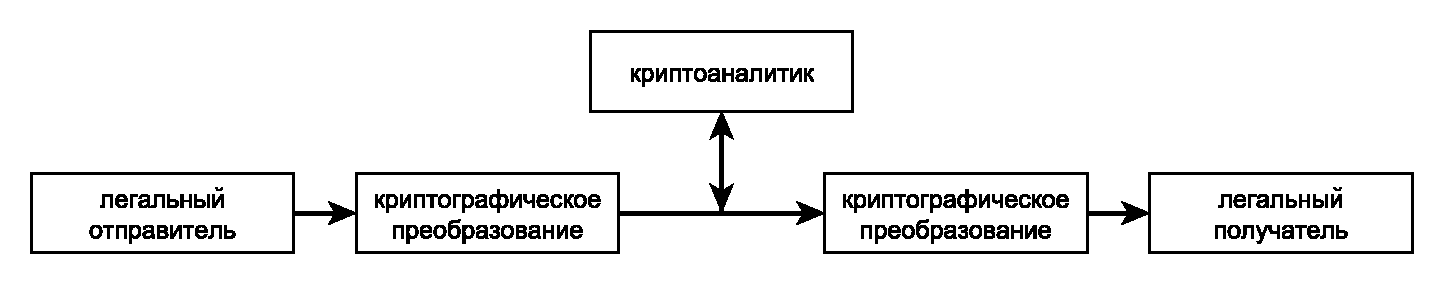
\includegraphics[width=1.0\textwidth]{pic/model-simple}
	\caption{Модель системы передачи информации с криптографической защитой по открытому каналу\label{pic:model-simple}}
\end{figure}

\begin{figure}[!thb]
	\centering
	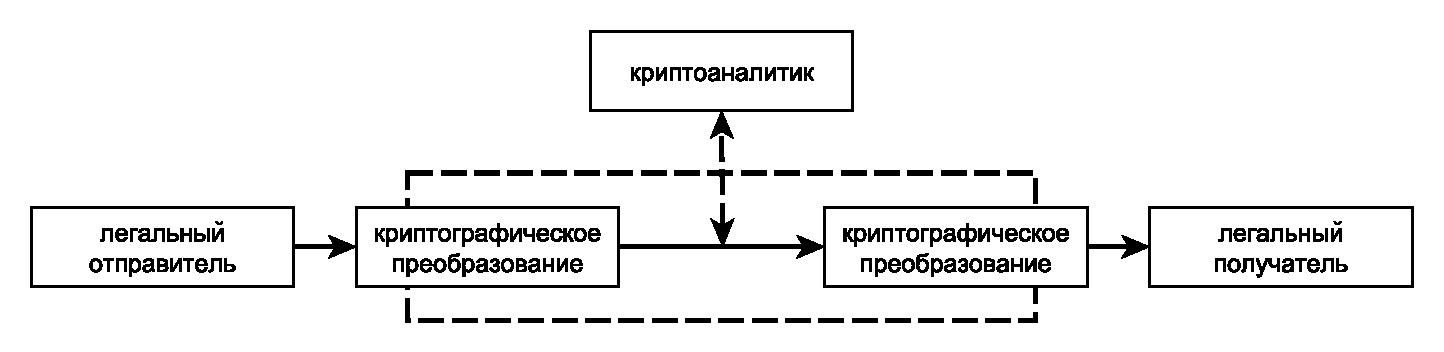
\includegraphics[width=1.0\textwidth]{pic/model-simple-with-channel}
	\caption{Открытый и защищённый каналы связи в модели системы передачи информации с криптографической защитой\label{pic:model-simple-with-channel}}
\end{figure}

Для обеспечения конфиденциальности информации используются криптографические системы с функцией шифрования. Пример системы с шифрованием показан на рис.~\ref{pic:model-cipher}.

\begin{figure}[!thb]
	\centering
	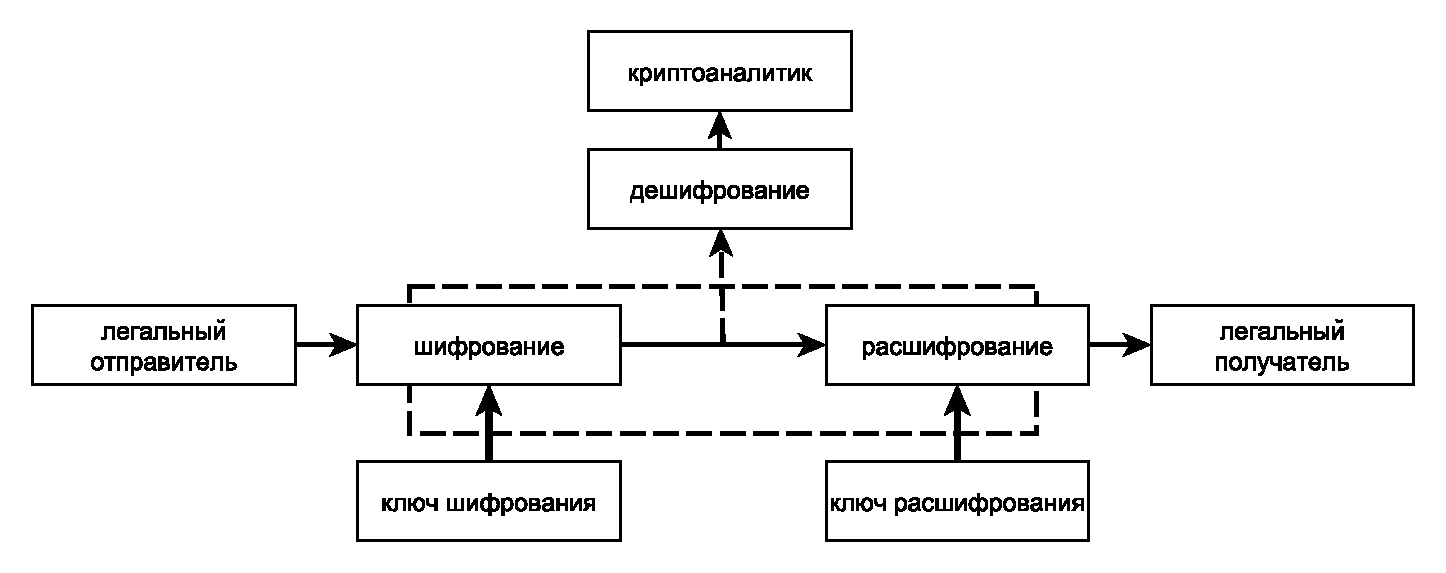
\includegraphics[width=1.0\textwidth]{pic/model-cipher}
	\caption{Модель системы передачи информации с шифрованием\label{pic:model-cipher}}
\end{figure}

Легальный отправитель \emph{шифрует} (\langen{cipher}) сообщение (\emph{открытый текст}\index{открытый текст}, \langen{plaintext}) с использованием \emph{ключа шифрования}\index{ключ!шифрования} (\langen{encryption key}) и передаёт зашифрованное сообщение (\emph{шифртекст}\index{шифртекст}, \langen{ciphertext, cyphertext} или \emph{шифрограмма}\index{шифрограмма}\footnote{Строго говоря, \emph{шифрограмма} -- это \emph{шифртекст} после его \emph{кодирования} для целей передачи по каналу связи.}) по открытому каналу связи. Легальный получатель \emph{расшифровывает} сообщение, используя \emph{ключ расшифрования}\index{ключ!расшифрования}, в общем случае отличающийся от ключа шифрования. Нелегальный пользователь, называемый криптоаналитиком, пытается \emph{дешифровать}\footnote{Обратите внимание, что в англоязычной литературе словом <<\textit{decryption}>> обозначается и расшифрование, и дешифрование.} сообщение, не имея ключа расшифрования, то есть нарушить конфиденциальность передаваемой информации. Можно сказать, что функции шифрования и расшифрования вместе с конкретными ключами шифрования и расшифрования помогли легальным участникам системы установить защищённый канал связи, обеспечивающий конфиденциальность информации.

\emph{Шифрование} (\emph{зашифрование}) -- это обратимое преобразование данных, формирующее шифртекст из открытого текста. \emph{Расшифрование} -- операция, обратная шифрованию. А вместе это \emph{шифр} -- криптографический метод, используемый для обеспечения конфиденциальности данных, включающий алгоритм зашифрования и алгоритм расшифрования.~\cite{GOST-89}

\emph{Шифр}\index{шифр} -- это множество обратимых функций отображения $E_{K_1}$\index{функция!шифрования} множества открытых текстов $\set{M}$ на множество шифртекстов $\set{C}$, зависящих от выбранного ключа шифрования $K_1$ из множества $\set{K}_E$, а также соответствующие им обратные функции расшифрования $D_{K_2}$, $\set{K}_D$, отображающие множество шифртекстов на множество открытых текстов:
\begin{equation}\label{eq:Encryption}\begin{array}{l}
	E_{k_1}, k_1 \in \set{K}_E: \set{M} \to \set{C}, \\
	D_{k_2}, k_2 \in \set{K}_D: \set{C} \to \set{M}, \\
	\forall k_1 \in \set{K}_E ~ \exists k_2 \in \set{K}_D: \\
	\forall m \in \set{M}: ~ E_{k_1} \left( m \right) = c, c \in \set{C}: \\
	D_{k_2} \left( c \right) = m.
\end{array}\end{equation}

Можно сказать, что шифрование -- это обратимая функция двух аргументов: сообщения и ключа. Обратимость -- основное условие корректности шифрования, по которому каждому зашифрованному сообщению $Y$ и ключу $K$ соответствует одно исходное сообщение $X$. Легальный пользователь $B$ (на приёмной стороне системы связи) получает сообщение $Y$ и осуществляет процедуру \emph{расшифрования}\index{расшифрование}.

Следует отличать \emph{шифрование} от \emph{кодирования}, будь то кодирование источника или канала. Под кодированием источника понимается преобразование информации для более компактного хранения, а под кодированием канала -- для повышения помехоустойчивости.

Модель системы передачи информации с обеспечением аутентичности передаваемых сообщений выглядит, как показано на рис.~\ref{pic:model-auten}.

\begin{figure}[!thb]
	\centering
	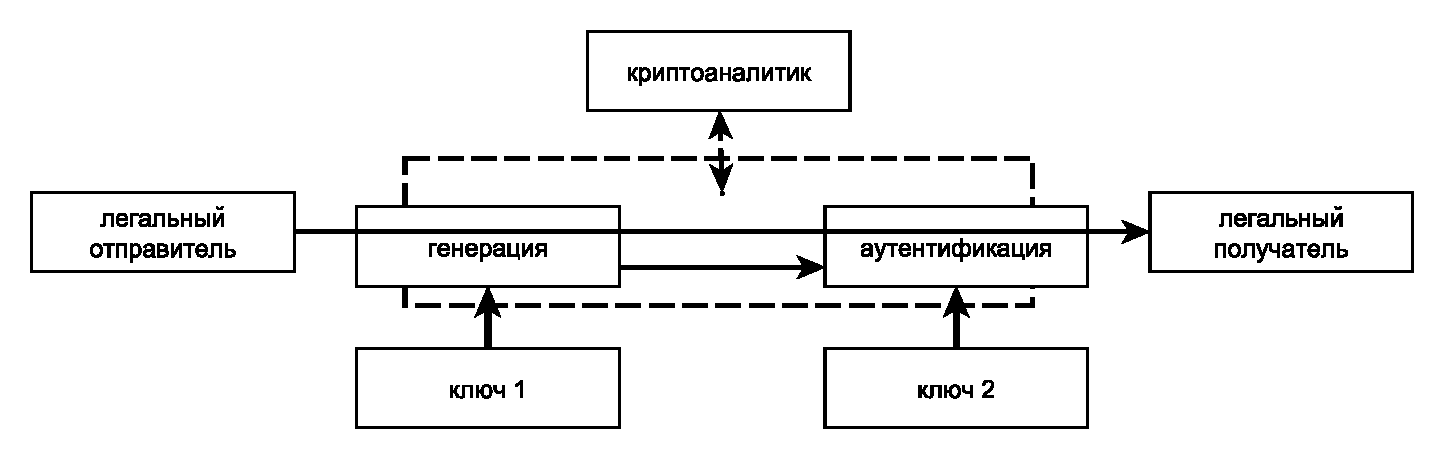
\includegraphics[width=1.0\textwidth]{pic/model-auten}
	\caption{Модель системы передачи информации с обеспечением аутентичности передаваемых сообщений\label{pic:model-auten}}
\end{figure}

В этой модели сообщение передаётся по открытому каналу связи без изменений (в открытом виде), однако вместе с сообщением от легального пользователя по тому же каналу связи передаётся дополнительная информация. Специальные криптографические методы позволяют гарантировать, что данную информацию может сформировать только легальный пользователь (или, в некоторых случаях, ещё и легальный получатель). Легальный получатель проверяет эту дополнительную информацию и убеждается, что сообщение пришло именно от легального отправителя и без изменений. Таким образом был организован защищённый канал связи с обеспечением аутентичности передаваемых сообщений. 

\index{канал связи!защищённый|)}\index{канал связи!открытый|)}


\section[Классификация]{Классификация криптографических механизмов}

\subsection{Симметричные и асимметричные криптосистемы}
\selectlanguage{russian}

Криптографические системы и шифры можно разделить на две большие группы в зависимости от принципа использования ключей для шифрования и расшифрования.

Если для шифрования и расшифрования используется один и тот же ключ $K$, либо если получение ключа расшифрования $K_2$ из ключа шифрования $K_1$ является тривиальной операцией, то такая криптосистема называется \emph{симметричной}\index{криптосистема!симметричная}. В зависимости от объёма данных, обрабатываемых за одну операцию шифрования, симметричные шифры делятся на \emph{блочные}\index{шифр!блочный}, в которых за одну операцию шифрования происходит преобразование одного блока данных (32 бита, 64, 128 или больше), и \emph{потоковые}\index{шифр!потоковый}, в которых работают с каждым символом открытого текста по отдельности (например, с 1 битом или 1 байтом). Примеры блочных шифров рассмотрены в главе~\ref{chapter-block-ciphers}, а потоковых -- в главе~\ref{chapter-stream-ciphers}.

Использование блочного шифра подразумевает разделение открытого текста на блоки одинаковой длины, к каждому из которых применяется функция шифрования. Кроме того, результат шифрования следующего блока может зависеть от предыдущего\footnote{Строго говоря, функция шифрования может применяться не только к самому блоку данных, но и к другим параметрам текущего отрывка открытого текста. Например, к его позиции в тексте (\langen{offset}) или даже к результату шифрования предыдущего блока.}. Данная возможность регулируется \emph{режимом работы блочного шифра}. Примеры нескольких таких режимов рассмотрены в разделе~\ref{section-block-chaining}.

Если ключ расшифрования получить из ключа шифрования вычислительно сложно, то такие криптосистемы называют криптосистемами \emph{с открытым ключом}\index{криптосистема!с открытым ключом} или \emph{асимметричными} криптосистемами\index{криптосистема!асимметричная}. Некоторые из них рассмотрены в главе~\ref{chapter-public-key}. Все используемые на сегодняшний день асимметричные криптосистемы работают с открытым текстом, составляющим несколько сотен или тысяч бит, поэтому классификация таких систем по объёму обрабатываемых за одну операцию данных не производится.

Алгоритм, который выполняет отображение аргумента произвольной длины в значение фиксированной длины, называется \emph{хеш-функцией}. Если для такой хеш-функции выполняются определённые свойства, например, устойчивость к поиску коллизий, то это уже \emph{криптографическая хеш-функция}. Такие функции рассмотрены в главе~\ref{chapter-hash-functions}.

Для проверки аутентичности сообщения с использованием общего секретного ключа отправителем и получателем используется \emph{код аутентификации [сообщения]} (другое название в русскоязычной литературе - \emph{имитовставка}, \langen{message authentication code, MAC}), рассмотренный в разделе~\ref{section-MAC}. Его аналогом в криптосистемах с открытым ключом является \emph{электронная подпись}, алгоритмы генерации и проверки которой рассмотрены в главе~\ref{chapter-public-key} вместе с алгоритмами асимметричного шифрования.

\subsection{Шифры замены и перестановки}

Шифры по способу преобразования открытого текста в шифртекст разделяются на шифры замены и шифры перестановки.

\input{substitution_ciphers}

\input{permutation_ciphers}

\input{composite_ciphers}

\subsection{Примеры современных криптографических примитивов}

Приведём примеры названий некоторых современных криптографических примитивов, из которых строят системы защиты информации.
\begin{itemize}
    \item DES\index{шифр!DES}, AES, ГОСТ 28147-89, Blowfish\index{шифр!Blowfish}, RC5\index{шифр!RC5}, RC6\index{шифр!RC6} -- блочные симметричные шифры, скорость обработки -- десятки мегабайт в секунду.
    \item A5/1, A5/2, A5/3\index{шифр!A5}, RC4\index{шифр!RC4} -- потоковые симметричные шифры с высокой скоростью. Семейство A5 применяется в мобильной связи GSM, RC4 -- в компьютерных сетях для SSL-соединения между браузером и веб-сервером.
    \item RSA\index{шифр!RSA} -- криптосистема с открытым ключом для шифрования.
    \item RSA\index{электронная подпись!RSA}, DSA\index{электронная подпись!DSA}, ГОСТ Р 34.10-2001\index{электронная подпись!ГОСТ Р 34.10-2001} -- криптосистемы с открытым ключом для электронной подписи.
    \item MD5\index{хеш-функция!MD5}, SHA-1\index{хеш-функция!SHA-1}, SHA-2\index{хеш-функция!SHA-2}, ГОСТ Р 34.11-94\index{хеш-функция!ГОСТ Р 34.11-94} -- криптографические хеш-функции.
\end{itemize}

\section{Методы криптоанализа и типы атак}
\selectlanguage{russian}

Нелегальный пользователь-криптоаналитик получает информацию путём дешифрования. Сложность этой процедуры определяется числом стандартных операций, которые надо выполнить для достижения цели. \emph{Двоичной сложностью}\index{сложность!двоичная} (или битовой сложностью) алгоритма называется количество двоичных операций, которые необходимо выполнить для его завершения.

Рассмотрим основные сценарии работы криптоаналитика $E$. В первом сценарии криптоаналитик может осуществлять подслушивание и (или) перехват сообщений. Его вмешательство не нарушает целостности информации: $Y=\widetilde{Y}$, где Y -- информация, как случайная величина, до вмешательства, $\widetilde{Y}$ -- после вмешательства. Эта роль криптоаналитика называется \emph{пассивной}. Так как он получает доступ к информации, то здесь нарушается конфиденциальность.

Во втором сценарии роль криптоаналитика \emph{активная}. Он может подслушивать, перехватывать сообщения и преобразовывать их по своему усмотрению: задерживать, искажать с помощью перестановок пакетов, устраивать обрыв связи, создавать новые сообщения и т.~п. В этом случае выполняется условие $Y \neq \widetilde{Y}$. Это значит, что одновременно нарушается целостность и конфиденциальность передаваемой информации.

Приведём примеры пассивных и активных атак:
\begin{itemize}
    \item Атака <<человек посередине>>\index{атака!<<человек посередине>>} (\langen{man-in-the-middle}) подразумевает криптоаналитика, который разрывает канал связи, встраиваясь между $A$ и $B$, получает сообщения от $A$ и от $B$, а от себя отправляет новые, фальсифицированные сообщения. В результате $A$ и $B$ не замечают, что общаются с $E$, а не друг с другом.
    \item Атака \emph{воспроизведения}\index{атака!воспроизведения} (\langen{replay attack}) предполагает, что криптоаналитик может записывать и воспроизводить шифртексты, имитируя легального пользователя.
    \item Атака на \emph{различение} сообщений\index{атака!на различение} означает, что криптоаналитик, наблюдая одинаковые шифртексты, может извлечь информацию об идентичности исходных открытых текстов.
    \item Атака на \emph{расширение} сообщений\index{атака!на расширение} означает, что криптоаналитик может дополнить шифртекст осмысленной информацией без знания секретного ключа.
    \item \emph{Фальсификация} шифртекстов\index{атака!фальсификацией} криптоаналитиком без знания секретного ключа.
\end{itemize}

Часто для нахождения секретного ключа криптоатаки строят в предположениях о доступности дополнительной информации. Приведём примеры:
\begin{itemize}
    \item Атака на основе известного открытого текста\index{атака!с известным открытым текстом} (\langen{chosen plaintext attack, CPA}) предполагает, что криптоаналитик имеет возможность выбирать открытый текст и получать для него соответствующий шифртекст.
    \item Атака на основе известного шифртекста\index{атака!с известным шифртекстом} (\langen{chosen ciphertext attack, CCA}) предполагает возможность криптоаналитику выбирать шифртекст и получать для него соответствующий открытый текст.
\end{itemize}

Обязательным требованием к современным криптосистемам является устойчивость ко всем известным типам атак: пассивным, активным и с дополнительной информацией.


%Приведём примеры возможных вариантов работы активного криптоаналитика.
%\begin{itemize}
%\item Криптоаналитик имеет $m$ шифрованных сообщений $Y_{1},Y_{2},\ldots Y_{m}$ и пытается определить ключ или прочитать открытый текст $X_{1},X_{2},\ldots X_{m}.$
%\item Криптоаналитик имеет несколько пар открытого и шифрованного текстов
%
%$(Y_{1},X_{1}),(Y_{2}X_{2}),\ldots (Y_{m}X_{m})$ и пытается дешифровать остальной текст или определить алгоритм шифрования или определить ключ.
%\item
%\item
%\item
%\end{itemize}

Для защиты информации от активного криптоаналитика и обеспечения её целостности дополнительно к шифрованию сообщений применяют имитовставку\index{имитовставка}. Для неё используют обозначение $\MAC$ (\langen{message authentication code}). Как правило, $\MAC$ строится на основе хеш-функций, которые будут описаны далее.

Существуют ситуации, когда пользователи $A$ и $B$ не доверяют друг другу. Например, $A$ -- банк, $B$ -- получатель денег. $A$ утверждает, что деньги были переведены, $B$ - что перевода не было. Решение задачи аутентификации и неотрицаемости состоит в обеспечении \emph{электронной подписью}\index{электронная подпись} каждого из абонентов. Предварительно надо решить задачу о генерировании и распределении секретных ключей.

В общем случае системы защиты информации должны обеспечивать:
\begin{itemize}
    \item конфиденциальность\index{конфиденциальность} (защиту от наблюдения),
    \item целостность\index{целостность} (защиту от изменения),
    \item аутентификацию (защиту от фальсификации пользователя и сообщений),
    \item доказательство авторства информации (доказательство авторства и защита от его отрицания)
\end{itemize}
как со стороны получателя, так и со стороны отправителя.

Важным критерием для выбора степени защиты является сравнение стоимости реализации взлома для получения информации и экономического эффекта от владения ей. Очевидно, что если стоимость взлома превышает ценность информации, взлом нецелесообразен.

%Сценарии защиты информации
%   Сценарий 1. A -- передающая сторона. B -- принимающая сторона. E -- пассивный
%криптоаналитик, который может подслушивать передачу, но не может вмешиваться
%в процесс передачи. Цель защиты: обеспечение конфиденциальности. Средства
%-- методы шифрования с секретным ключом (симметричные системы шифрования)
%и методы шифрования с открытым ключом (асимметричные системы шифрования).
%Сценарий 2. E -- активный криптоаналитик, который может изменять, удалять и вставлять
%сообщения или их части. Цель защиты -- обеспечение конфиденциальности (не
%всегда) и обеспечение целостности. Средства -- методы шифрования и добавление
%имитовставки\index{имитовставка} (Message Authentication Code -- $\MAC$).
%Сценарий 3. A и B не доверяют друг другу. Цель защиты -- аутентификация пользователя.
%Средства -- электронная подпись.


\input{The_minimum_key_lengths}


\input{writing-rules}

\section{Свойства безопасности протоколов}
\selectlanguage{russian}
Защищённая система и, соответственно, защищённый протокол могут выполнять разные функции безопасности. Многие из этих функций или целей (\langen{{goals}}) можно сформулировать как устойчивость к определённому классу атак. Наиболее полным и актуальным считается перечисление и толкование этих целей в документе проекта AVISPA (\langen{Automated Validation of Internet Security Protocols and Applications})~\cite{AVISPA:2003}, суммирующим описания из различных документов IETF (\langen{{Internet Engineering Task Force}}). Данные цели принято считать \emph{формализируемыми} -- то есть такими, что для отдельных протоколов есть возможность формально доказать или опровергнуть достижение этих целей.

\begin{itemize}
	\item Аутентификация (однонаправленная).\\*
		\langen{Authentication (unicast)}.
	\begin{itemize}
		\item[(G1)] Аутентификация субъекта.\\*
			\langen{Entity authentication (Peer Entity Authentication)}.
		\item[{}] Гарантия для одной стороны протокола через представление доказательств и / или учётных данных второй стороны, участвующей в протоколе, и того, что вторая сторона действительно участвовала в текущем сеанса протокола. Обычно делается через представления таких данных, которые могли быть сгенерированы только второй стороной. Аутентификация субъекта подразумевает, что полученные данные могут быть однозначно прослежены до субъекта протокола, что подразумевает аутентификацию источника данных.
		\item[(G2)] Аутентификация сообщения.\\*
			\langen{Message authentication (Data Origin Authentication)}.
		\item[{}] Гарантия того, что полученное сообщение или фрагмент данных были созданы определённым субъектом в какое-то (обычно неуказанное) время в прошлом, и что эти данные не были повреждены или подделаны. Но без предоставления уникальности или своевременности. Аутентификация сообщений подразумевает их целостность.
		\item[(G3)] Защита от повтора.\\*
			\langen{Replay Protection}.
		\item[{}] Защита от ситуации, когда некоторая сторона запишет некоторое сообщение и воспроизведёт его позднее (возможно -- в другом сеансе протокола), что приведёт к некорректной интерпретации данной стороны как аутентифицированной.
	\end{itemize}

	\item Аутентификация при рассылке по многим адресам или при подключении к службе подписки/уведомления.\\*
		\langen{Authentication in Multicast or via a Subscribe / Notify Service}.
	\begin{itemize}
		\item[(G4)] Неявная аутентификация получателя.\\*
			\langen{Implicit Destination Authentication}.
		\item[{}] Протокол должен гарантировать, что отправленное сообщение доступно для чтения только легальным получателям. То есть, только легальные авторизованные участники будут иметь доступ к актуальной информации, многоадресному сообщению или сеансу групповой связи. Включает в себя группы рассылки с очень динамичным членством.
		\item[(G5)] Аутентификация источника.\\*
			\langen{Source Authentication}.
		\item[{}] Легальные получатели смогут аутентифицировать источник и содержание информации или группового общения. Включает случаи, когда члены группы не доверяют друг другу.
	\end{itemize}

	\item[(G6)] Авторизация (третьей доверенной стороной).\\*
		\langen{Authorization (by a Trusted Third Party)}.
	\item[{}] Гарантия возможности авторизовать (в терминах протокола) одного субъекта на доступ к ресурсу другого с помощью третьей доверенной стороны. Подразумевает, что владелец ресурса может не иметь собственных списков доступа (\langen{Access Control List, ACL})) и полагается на таковые у доверенной стороны.

	\item Совместная генерация ключа.\\*
		\langen{Key Agreement Properties}.
	\begin{itemize}
		\item[(G7)] Аутентификация ключа.\\*
			\langen{Key authentication}.
		\item[{}] Гарантия для одного из субъектов, что только легальные пользователи могут получить доступ к конкретному секретному ключу.
		\item[(G8)] Подтверждение владения ключом.\\*
			\langen{Key confirmation (Key Proof of Possession)}.
		\item[{}] Гарантия для одного из субъектов, что другой субъект действительно владеет конкретным секретным ключом (либо информацией, необходимой для получения такого ключа).
		\item[(G9)] Совершенная прямая секретность.\\*
			\langen{Perfect Forward Secrecy (PFS)}.
		\item[{}] Гарантия того, что компрометация мастер-ключей в будущем не приведёт к компрометации сессионных ключей уже прошедших сеансов протокола.
		\item[(G10)] Формирование новых ключей.\\*
			\langen{Fresh Key Derivation}.
		\item[{}] Гарантия возможности создать новые сессионные ключи для каждого сеанса протокола. 
		\item[(G11)] Защищённая возможность договориться о параметрах безопасности.\\*
			\langen{Secure capabilities negotiation (Resistance against Downgrading and Negotiation Attacks)}.
		\item[{}] Гарантия не только того, что легальные стороны имеют возможность договориться о параметрах безопасности, но и того, что нелегальная сторона не вмешалась в протокол и не привела к выбору предпочтительных ей (возможно -- наиболее слабых) параметров безопасности.
	\end{itemize}

	\item[(G12)] Конфиденциальность (секретность).\\*
		\langen{Confidentiality (Secrecy)}.
	\item[{}] Гарантия, что конкретный элемент данных (часть передаваемого сообщения) остаётся неизвестным для злоумышленника. В данной цели не рассматривается секретность сеансового ключа, проверка подлинности ключа или надёжность долговременных мастер-ключей.

	\item Анонимность.\\*
		\langen{Anonymity}.
	\begin{itemize}
		\item[(G13)] Защита идентификаторов от прослушивания (несвязываемость).\\*
			\langen{Identity Protection against Eavesdroppers}.
		\item[{}] Гарантия, что злоумышленник (подслушивающий) не в состоянии связать обмен сообщениями субъектом с его реальной личностью.
		\item[(G14)] Защита идентификаторов от других участников.\\*
			\langen{Identity Protection against Peer}.
		\item[{}] Гарантия, что участник переписки не в состоянии связать обмен сообщениями субъекта с реальной личностью, но только с некоторым псевдонимом.
	\end{itemize}

	\item[(G15)] Ограниченная защита от атак отказа в обслуживании.\\*
		\langen{(Limited) Denial-of-Service (DoS) Resistance}.
	\item[{}] Гарантия, что протокол следует определённым принципам, уменьшающих вероятность (усложняющих использование) отдельных классов атак отказа в обслуживании.

	\item[(G16)] Неизменность отправителя.\\*
		\langen{Sender Invariance}.
	\item[{}] Гарантия для одной из сторон, что источник сообщения остался таким же, как тот, который начал общение, хотя фактическая идентификация источника не важна для получателя.

	\item Неотрекаемость.\\*
		\langen{Non-repudiation}.
	\begin{itemize}
		\item[(G17)] Подотчётность.\\*
			\langen{Accountability}.
		\item[{}] Гарантия возможности отслеживания действий субъектов над объектами.
		\item[(G18)] Доказательство происхождения.\\*
			\langen{Proof of Origin}.
		\item[{}] Гарантия неопровержимости доказательств источника сообщения.
		\item[(G19)] Доказательство доставки.\\*
			\langen{Proof of Delivery}.
		\item[{}] Гарантия неопровержимости доказательств факта получения сообщения.
	\end{itemize}

	\item[(G20)] Защищённое временное свойство.\\*
		\langen{Safety Temporal Property}.
	\item[{}] Гарантия возможности доказать, что факт нахождения системы в одном из состояний означает, что некогда в прошлом система хотя бы раз находилась в некотором другом состоянии. Например, что получение субъектом доступа к ресурсу означает, что некогда в прошлом субъект успешно оплатил данный доступ.

\end{itemize}

Примеры свойств безопасности, реализуемыми различными протоколами приведены в таблице~\ref{tab:protocols-properties}).

\begin{landscape}
{\renewcommand{\arraystretch}{1.5}
\begin{table}
    \centering
    \begin{tabular}{|l|c|c|c|c|c|c|c|c|c|c|c|c|c|c|c|}
        \hline
Протокол \textbackslash Цель G & 1 & 2 & 3 & 4 & 5 & 6 & 7 & 8 & 9 & 10 & 11 & 12 & 13 & 14 & 15 \\
        \hline
        EAP-IKEv2              & × & × & × &   &   & × & × &   &   &  × &    &    &    &    &  × \\
        \hline
        EKE                    & × & × &   &   &   &   &   &   &   &    &    &  × &    &    &    \\
        \hline
        IKE                    & × & × & × &   &   &   & × &   & × &  × &  × &    &  × &  × &  × \\
        \hline
        IKEv2                  & × & × & × &   &   &   & × &   & × &  × &  × &    &    &    &  × \\
        \hline
        DHCP-IPSec-tunnel      & × & × &   &   &   &   &   &   &   &    &    &  × &    &    &    \\
        \hline
        kerberos               & × & × & × &   &   & × & × &   &   &  × &    &    &    &    &    \\
        \hline
        SSH                    & × & × & × &   &   &   & × &   &   &  × &  × &    &    &    &    \\
        \hline
        TLS, TLS 1.1, TLS 1.2  & × & × & × &   &   &   & × &   &   &  × &  × &    &  × &    &    \\
        \hline
        TLS 1.3                & × & × & × &   &   &   & × &   & × &  × &  × &    &  × &    &    \\
        \hline
        SET                    & × & × & × &   &   &   &   &   &   &    &    &    &  × &    &    \\
        \hline
    \end{tabular}
    \caption{Примеры свойств безопасности протоколов (по \cite{Cheremushkin:2009} с дополнениями).}
    \label{tab:protocols-properties}
\end{table}
}
\end{landscape}


\section{Классификация протоколов}\label{section-protocols-classification}
\selectlanguage{russian}

Общепризнанная классификация защитных протоколов отсутствует. Однако можно выделить набор \emph{объективных и однозначных} признаков, классифицирующих протоколы.

\begin{itemize}
    \item Классификация по числу участников протокола:
    \begin{itemize}
        \item двусторонний\index{протокол!двусторонний}, 
        \item трёхсторонний\index{протокол!трёхсторонний} и т.~п., 
        \item многосторонний\index{протокол!многосторонний}.
    \end{itemize}
    \item Классификация по числу передаваемых сообщений:
    \begin{itemize}
        \item интерактивный\index{протокол!интерактивный} (с наличием взаимного обмена сообщениями);
        \item неинтерактивный\index{протокол!неинтерактивный}, в котором участники обмениваются по одному сообщению, причём их содержание не зависит друг от друга. Также называется \emph{схемами}\index{схема}\footnote{Определение не совсем полное. Любая схема предполагает как минимум два этапа. На первом предварительном этапе доверенный центр распределяет некоторую информацию между одноранговыми участниками. На втором этапе (конкретные сеансы протокола) участники обмениваются этой информацией, получая исходный секрет или новый секретный сеансовый ключ. Причём обмен информацией может идти более чем между двумя участниками. Однако после взаимного обмена информацией дополнительных проходов для выполнения целей схемы не требуется.}.
    \end{itemize}
    \item Классификация по числу проходов (раундов):
    \begin{itemize}
        \item двупроходной (двураундовый),
        \item трёхпроходной (трёхраундовый) и т.~д.,
        \item многопроходной (многораундовый) или циклический.
    \end{itemize}
    \item Классификация по используемым криптографическим системам:
    \begin{itemize}
        \item на основе только симметричных\index{криптосистема!симметричная} криптосистем;
        \item на основе в том числе асимметричных\index{криптосистема!асимметричная} криптосистем.
    \end{itemize}
    \item Классификация по защищённым свойствам протокола:
    \begin{itemize}
        \item[(G1)] обеспечивает или нет аутентификацию первой, второй стороны протокола и т.~д.;
        \item[(G2)] обеспечивает или нет аутентификацию сообщений;
        \item[(G3)] обеспечивает или нет защиту от повторов;
        \item[{}] и т.~п.
    \end{itemize}
    \item Классификация по типам участников:
    \begin{itemize}
        \item одноранговый, когда все участники в рамках протокола могут выполнять произвольные роли;
        \item с доверенным посредником, когда в протоколе всегда участвует третья доверенная сторона;
        \item с доверенным арбитром, когда в протоколе может участвовать третья доверенная сторона, но только в отдельных случаях, когда остальные участники не пришли к согласию.
    \end{itemize}
\end{itemize}

Можно также ввести менее объективную и однозначную классификацию, основываясь на субъективной оценке протоколов.
\begin{itemize}
    \item Классификация по целевому назначению протокола:
    \begin{itemize}
        \item \dots обеспечения целостности, 
        \item \dots цифровой подписи, 
        \item \dots идентификации, 
        \item \dots конфиденциальности, 
        \item \dots распределения ключей, 
        \item \dots и~т.~п.
    \end{itemize}
    \item Классификация по <<полноте>> выполняемых функций:
    \begin{itemize}
        \item примитивные, используются как базовый компонент при построении прикладных протоколов;
        \item промежуточные;
        \item прикладные, предназначены для решения практических задач.
    \end{itemize}
\end{itemize}

Классификацию по целевому предназначению можно также переформулировать в виде классификации по защищённым свойствам протокола, для обеспечения которых он разрабатывался. При этом нужно будет выделить <<основные свойства>> (например, G10 -- формирование новых ключей), а большую часть остальных отнести к дополнительным (например, G7 -- аутентификация ключа, и G8 -- подтверждение владения ключом). Определение того, какие именно из свойств <<основные>>, а какие <<дополнительные>>, будет создавать неоднозначность классификации по целевому назначению протокола. Если же все свойства протокола назвать <<основными>>, то такая классификация станет слишком детальной.

Классификация по <<полноте>> выполняемых функций проблематична из-за того, что ни один протокол нельзя назвать в полной мере <<прикладным>>. Любой протокол сам по себе это лишь часть некоторой информационной (или организационной) системы, которая как раз и выполняет требуемую пользователями функцию. Однако можно говорить о том, что отдельные протоколы (например, TLS\index{протокол!TLS}) являются протоколами более высокого уровня, чем протоколы, например, Диффи~---~Хеллмана\index{протокол!Диффи~---~Хеллмана}, так как последний часто выступает составной частью того же протокола TLS.


\section{Атаки на протоколы}\label{section-protocols-attacks}
\selectlanguage{russian}

Защищённые свойства протоколов могут быть заявленными, когда о них заявляют сами авторы протокола (и, обычно, приводят различные аргументы в пользу выполнения данных функций), и подразумеваемыми, когда авторы некоторой системы рассчитывают на реализацию защищённых свойств некоторым протоколом.

Под \emph{атакой на защищённый протокол}\index{атака!на протокол} понимается попытка проведения анализа сообщений протокола и/или выполнения не\-пред\-усмотренных протоколом действий (уничтожение, дублирование или генерация и посылка сообщений) для нарушения заявленных или подразумеваемых свойств протокола.\footnote{Используется модифицированное определение из~\cite{Cheremushkin:2009}. Отличие в том, что Черёмушкин в своём определении не описывает, что такое <<нарушение работы протокола>> и оставляет двусмысленными случаи нарушения, например, свойств G9/PFS и G20/STP.}

Атака считается \emph{успешной}, если нарушено хотя бы одно из заявленных или подразумеваемых свойств протокола.

В случае успешной атаки на подразумеваемые свойства будем уточнять, что успешна \emph{атака на использование протокола} в некоторой системе. Это будет говорить, разумеется, не о недостатках самого протокола, но о неверном выборе протокола (или его настроек) авторами системы.

Существует большое количество типов атак на протоколы. У многих атак есть некоторые общие принципы, что позволяет выделить классы атак для упрощения анализа и разработки протоколов, устойчивых к целым классам атак.

\begin{itemize}
    \item[MITM] Атака <<человек посередине>>\index{атака!<<человек посередине>>}\\*
        \langen{man-in-the-middle attack}
    \item[{}] Класс атак, в котором злоумышленник ретранслирует и, при необходимости, изменяет все сообщения, проходящие между двумя и более участниками протокола, причём последние не знают о существовании злоумышленника, считая, что общаются непосредственно друг с другом. К данной атаке уязвимы все протоколы, которые не реализуют взаимную аутентификацию сторон (цель G1). Классическим примером атаки данного класса является атака на протокол Диффи~---~Хеллмана\index{протокол!Диффи~---~Хеллмана}, рассмотренном в разделе~\ref{section-protocols-diffie-hellman}.

    \item[Replay] Атака с повторной передачей\\*
        \langen{replay attack}
    \item[{}] Класс атак, в котором злоумышленник записывает все сообщения, проходящие в одном сеансе протокола, а далее повторяет их в новом, выдавая себя за одного из участников первого сеанса. Примерами протоколов, к которым применима данная атака, являются протоколы Ву~---~Лама\index{протокол!Ву~---~Лама} и бесключевой протокол Шамира\index{протокол!Шамира бесключевой} из раздела~\ref{section-protocols-shamir}.

    \item[TF] Атака подмены типа\\*
        \langen{type flaw attack}
    \item[{}] Класс атак, в котором злоумышленник используя переданное в легальном сеансе протокола сообщение конструирует новое, передавая его на другом проходе (раунде) протокола под видом сообщения другого типа (с другим предназначением). К таким атакам уязвимы, например, протоколы Wide-Mouth Frog\index{протокол!Wide-Mouth Frog} из раздела~\ref{section-protocols-wide-moth-frog}, Деннинга~---~Сакко\index{протокол!Деннинга~---~Сакко}, Отвей~---~Рииса\index{протокол!Отвей~---~Рииса}, а также некоторые варианты протокола Yahalom\index{протокол!Yahalom}.

    \item[PS] Атака с параллельными сеансами\\*
        \langen{parallel-session attack}
    \item[{}] Класс атак, в котором злоумышленник инициирует несколько одновременных сеансов протокола с целью использования сообщений из одного сеанса в другом. Примером протокола, уязвимого к данному классу атак, является симметричный вариант протокола Нидхема~---~Шрёдера\index{протокол!Нидхема~---~Шрёдера}, рассмотренном в разделе~\ref{section-protocols-needham-schroeder}.

    \item[STS] Атака с известным разовым ключом\index{атака!с известным разовым ключом}\\*
        \langen{short-term secret attack}
    \item[KN] Атака с известным сеансовым ключом\index{атака!с известным сеансовым ключом}\\*
        \langen{known-key attack}
    \item[{}] Классы атак, в которых злоумышленник получает доступ к временным секретам, используемых в протоколах (например, новым сеансовым ключам), после чего может обеспечить, например, аутентификацию или хотя бы установление сессии от имени одной из сторон протокола.

    \item[UKS] Атака с неизвестным сеансовым ключом\\*
        \langen{unknown key-share attack}
    \item[{}] Класс атак на протоколы с аутентификацией ключа, в которых злоумышленник получает возможность доказать одной из сторон владение ключом (с помощью, например, повтора сообщения из легального сеанса), хотя сам ключ злоумышленник не знает. К такому классу атак уязвим, например, симметричный протокол Нидхема-Шрёдера из раздела~\ref{section-protocols-needham-schroeder}.

\end{itemize}

Важно отметить, что если не сказано иное, то в рамках анализа криптографических протоколов (не конкретных систем) используется предположение о стойкости всех используемых криптографических примитивов. Например, предполагается, что пока идёт защищённый обмен информацией, использующий сеансовый ключ, выработанный в сеансе некоторого криптографического протокола, то злоумышленнику не хватит ресурсов и времени на то, чтобы получить данный сеансовый ключ через атаку на используемые шифры или криптографически-стойкие хеш-функции.

С другой стороны, следует предполагать, что сеансовые ключи, получаемые в рамках сеансов протоколов, через некоторое время (однако, много большее времени самого сеанса связи) будут получены злоумышленником (классы атак STS и KN). Много позднее, возможно, злоумышленник сможет получить доступ и к <<мастер>>-ключам длительного использования, так что протоколы с генерацией сеансовых ключей должны разрабатываться в том числе со свойством G9/PFS.


\chapter{Распространение ключей}\label{chapter-key-distribution-protocols}

Задача распространения ключей является одной из множества задач построения надёжной сети общения многих абонентов. Задача состоит в получении в нужный момент времени двумя легальными абонентами сети секретного сессионного ключа шифрования (и аутентификации сообщений). Хорошим решением данной задачи будем считать такой протокол распространения ключей, который удовлетворяет следующим условиям.

\begin{itemize}
	\item В результате работы протокола между двумя абонентами должен быть сформирован секретный сессионный ключ.
	\item Успешное окончание протокола в том числе должно означать и успешную взаимную аутентификацию абонентов. Не должно быть такого, что протокол успешно завершился с точки зрения одной из сторон, а вторая сторона при этом представлена злоумышленником.
	\item К участию в работе протокола должны допускаться только легальные пользователи сети. Внешний пользователь не должен иметь возможность получить общий сессионный ключ с кем-либо из абонентов.
	\item Добавление нового абонента в сеть (или исключение из неё) не должно требовать уведомления всех участников сети.
\end{itemize}

Последнее требование сразу исключает такие варианты протоколов, в которых каждый из абонентов знал бы некоторый мастер-ключ общения с любым другим участником. Данные варианты плохи тем, что с ростом системы количество пар мастер-ключей <<абонент-абонент>> растёт как квадрат от количества участников. Поэтому большая часть рассматриваемых решений состоит в том, что в сети выделяется один или несколько доверенных центров T (\langen{Trent}, от \langen{trust}), которые как раз и владеют информацией обо всех легальных участниках сети и их ключах. Они же будут явно или неявно выступать одним из участников протоколов по формированию сеансовых ключей.

\begin{figure}[!htb]
    \centering
    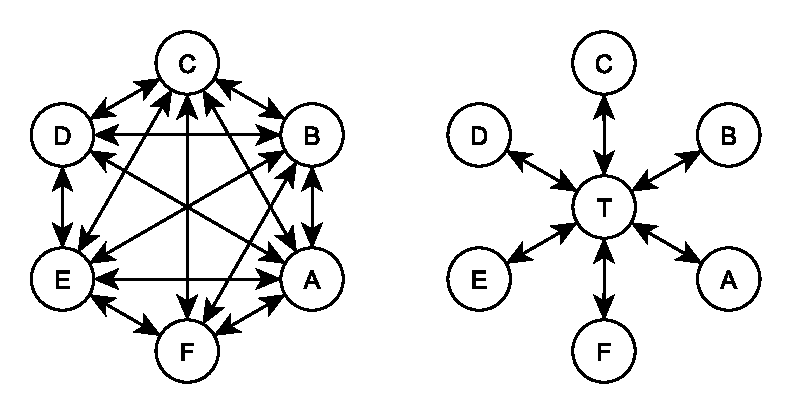
\includegraphics[width=0.8\textwidth]{pic/key_distribution-networks}
    \caption{Варианты сетей без выделенного доверенного центра и с выделенным доверенным центром T\label{fig:key_distribution-networks}}
\end{figure}

Если говорить о требованиях к данному классу протоколов с точки зрения свойств безопасности, то <<идеальный>> протокол распространения ключей должен реализовывать следующие цели:
\begin{itemize}
    \item[G1] аутентификация сторон протокола;
    \item[G3] защита от повтора;
    \item[G7] аутентификация ключа;
    \item[G8] подтверждение владения [новым] ключом;
    \item[G9] совершенная прямая секретность;
    \item[G10] формирование новых ключей.
    \item[G11] ограниченная защита от атак отказа в обслуживании.
\end{itemize}

Разумеется, <<идеальный>> протокол должен быть устойчивым ко всем известным атакам, в том числе рассмотренным в разделе~\ref{section-protocols-attacks}.

\subimport*{symmetric/}{index}

\section{Трёхпроходные протоколы}\label{section-three-pass-protocols}
\selectlanguage{russian}

Если между Алисой и Бобом существует канал связи, недоступный для модификации злоумышленником (то есть когда применима модель только пассивного криптоаналитика), то даже без предварительного обмена секретными ключами или другой информацией можно воспользоваться идеями, использованными ранее в криптографии на открытых ключах. После описания RSA в 1978 году, в 1980 Ади Шамир предложил использовать криптосистемы, основанные на коммутативных операциях, для передачи информации без предварительного обмена секретными ключами. Если предположить, что передаваемой информацией является выработанный одной из сторон секретный сеансовый ключ, то в общем виде мы получаем следующий трёхпроходной протокол.

\begin{figure}[thb]
	\centering
	\begin{sequencediagram}
		\newinst{Alice}{Alice}
		\newinst[2.5]{Bob}{Bob}

		\mess{Alice}{$  E_A \left( K \right) $}{Bob}
		\mess{Bob}{$ E_B \left( E_A \left( K \right) \right) $}{Alice}
		\mess{Alice}{$ E_B \left( K \right) $}{Bob}
	\end{sequencediagram}
	\caption{Диаграмма последовательности взаимодействия участников в трёхпроходных протоколах\label{fig:key_distribution-three-pass}}
\end{figure}

Предварительно:

\begin{itemize}
	\item Алиса и Боб соединены незащищённым каналом связи, открытым для прослушивания (но не для модификации) злоумышленником.
	\item Каждая из сторон имеет пару из открытого и закрытого ключей $K_A$, $k_A$, $K_B$, $k_B$ соответственно.
	\item Сторонами выбрана и используется коммутативная функция шифрования:
	\[\begin{array}{lll}
		D_{A} \left( E_{A} \left( X \right) \right)	= X                                       & \forall X, \left\{ K_A, k_a \right\}; \\
		E_{A} \left( E_{B} \left( X \right) \right)	= E_B \left( E_A \left( X \right) \right) & \forall ~ K_A, K_B, X.
	\end{array}\]
\end{itemize}

Диаграмма последовательности взаимодействия участников протокола показана на рис.~\ref{fig:key_distribution-three-pass}. Протокол состоит из трёх проходов с передачей сообщений (отсюда название) и одного заключительного, на котором Боб вычисляет сеансовый ключ.

\begin{protocol}
    \item[(1)] Алиса выбирает новый сеансовый ключ $K$
    \item[{}] $Alice \to \left\{ E_A \left( K \right) \right\} \to Bob$
    \item[(2)] $Bob \to \left\{ E_B \left( E_A \left( K \right) \right) \right\} \to Alice$
    \item[(3)] Алиса, используя коммутативность функции шифрования, <<исключает>> из сообщения Боба шифрование на своём ключе $K_A$:
	\[ D_A \left( E_B \left( E_A \left( K \right) \right) \right) = D_A \left( E_A \left( E_B \left( K \right) \right) \right) = E_B \left( K \right). \]
    \item[{}] $Alice \to \left\{ E_B \left( K \right) \right\} \to Bob$
    \item[(4)] Боб расшифровывает $D_B \left( E_B \left( K \right) \right) = K$
\end{protocol}

В результате работы протокола стороны получают общий секретный ключ $K$.

Общим недостатком всех подобных протоколов является отсутствие аутентификации сторон. Конечно, в случае пассивного криптоаналитика это не требуется, но в реальной жизни всё-таки нужно рассматривать все возможные модели (в том числе активного криптоаналитика) и использовать такие протоколы, которые предполагают взаимную аутентификацию сторон.

Также, в отличие, например, от схемы Диффи~---~Хеллмана, рассмотренной в разделе~\ref{section-protocols-diffie-hellman}, новый ключ выбирается инициатором сеанса. Это позволяет инициатору, исходя не из лучших побуждений, заставить второго участника использовать устаревший сеансовый ключ.

Если говорить в терминах свойств безопасности, то все представители данного класса протоколов декларируют только аутентификацию ключа (G7). В отличие от схемы Диффи~---~Хеллмана, трёхпроходные протоколы не требуют выбора новых <<мастер>>-ключей для каждого сеанса протокола, из-за чего нельзя гарантировать ни совершенную прямую секретность (G9), ни формирование новых ключей (G10).

\subsection{Тривиальный вариант}

Приведём пример протокола на основе функции XOR (побитовое сложение по модулю 2). Хотя данная функция может использоваться как фундамент для построения систем совершенной криптостойкости (см. главу~\ref{chapter:perfect_secure_systems}), для трёхпроходного протокола это неудачный выбор. Продемонстрируем это далее.

Пусть перед началом протокола обе стороны имеют свои секретные ключи $K_A$ и $K_B$, представляющие собой случайные двоичные последовательности с равномерным распределением символов. Функция шифрования определяется как $E_i( X ) = X \oplus K_i$, где $X$ это сообщение, а $K_i$ -- секретный ключ. Очевидно, что:

\[ \begin{matrix}
\forall i, j, X: E_i \left( E_j \left( X \right) \right) & = & X \oplus K_j \oplus K_i & = & \\ 
 & = & X \oplus K_i \oplus K_j & = & E_j \left( E_i \left( X \right) \right).
\end{matrix}
\]

Протокол состоит из следующих проходов и действий.

\begin{figure}[thb]
	\centering
	\begin{sequencediagram}
		\newinst{Alice}{Alice}
		\newinst[2.5]{Bob}{Bob}
		
		\mess{Alice}{$  K \oplus K_A $}{Bob}
		\mess{Bob}{$ K \oplus K_A \oplus K_B $}{Alice}
		\mess{Alice}{$ K \oplus K_B $}{Bob}
	\end{sequencediagram}
	\caption{Диаграмма последовательности взаимодействия участников в тривиальном трёхпроходном протоколе}
\end{figure}

\begin{protocol}
    \item[(1)] Алиса выбирает новый сеансовый ключ $K$
    \item[{}] $Alice \to \left\{ E_A \left( K \right) = K \oplus K_A \right\} \to Bob$
    \item[(2)] $Bob \to \left\{ E_B \left( E_A \left( K \right) \right) = K \oplus K_A \oplus K_B \right\} \to Alice$
    \item[(3)] Алиса, используя коммутативность функции шифрования,
	\[ D_A \left( E_B \left( E_A \left( K \right) \right) \right) = K \oplus K_A \oplus K_B \oplus K_A = K \oplus K_B = E_B \left( K \right). \]
    \item[{}] $Alice \to \left\{ E_B \left( K \right) = K \oplus K_B \right\} \to Bob$
    \item[(4)] Боб расшифровывает $D_B \left( E_B \left( K \right) \right) = K \oplus K_B \oplus K_B = K$
\end{protocol}

По окончании сеанса протокола Алиса и Боб знают общий сеансовый ключ $K$.

Предложенный выбор коммутативной функции шифрования совершенной секретности является неудачным, так как существуют ситуации, при которых криптоаналитик может определить ключ $K$. Предположим, что криптоаналитик перехватил все три сообщения:
    \[ K \oplus K_A, ~~ K \oplus K_A \oplus K_B, ~~ K \oplus K_B. \]
Сложение по модулю 2 всех трёх сообщений даёт ключ $K$. Поэтому такая система шифрования не применяется.

Теперь приведём протокол надёжной передачи секретного ключа, основанный на экспоненциальной (коммутативной) функции шифрования. Стойкость этого протокола связана с трудностью задачи вычисления дискретного логарифма: при известных значениях $y, g, p$, найти $x$ из уравнения $y = g^x \bmod p$.

\subsection{Бесключевой протокол Шамира}\index{протокол!Шамира бесключевой|(}\label{section-protocols-shamir}

Стороны предварительно договариваются о большом простом числе $p \sim 2^{1024}$. Каждая из сторон выбирает себе по секретному ключу $a$ и $b$. Эти ключи меньше и взаимно просты с $p-1$. Также стороны приготовили по специальному числу $a'$ и $b'$, которые позволяют им расшифровать сообщение, зашифрованное своим ключом:
\[\begin{array}{l}
a' = a{-1} \mod (p-1), \\
a \times a' = 1 \mod (p-1), \\
\forall X: (X^a)^{a'} = X. \\
\end{array}\]

Последнее выражение верно по следствию из малой теоремы Ферма\index{теорема!Ферма малая}. Операции шифрования и расшифрования определяются следующим образом:
\[\begin{array}{lll}
\forall M < p: & C = E( M ) = M^{a}            & \mod p, \\
               & D( C ) = C^{a'}               & \mod p, \\
               & D_A( E_A( M ) ) = M^{aa'} = M & \mod p. \\
\end{array}\]

\begin{figure}[thb]
	\centering
	\begin{sequencediagram}
		\newinst{Alice}{Alice}
		\newinst[2.5]{Bob}{Bob}

		\mess{Alice}{$ K^a \bmod p $}{Bob}
		\mess{Bob}{$ K^{ab} \bmod p $}{Alice}
		\mess{Alice}{$ K^b \bmod p $}{Bob}
	\end{sequencediagram}
	\caption{Диаграмма последовательности взаимодействия участников в бесключевом протоколе Шамира}
\end{figure}

\begin{protocol}
    \item[(1)] Алиса выбирает новый сеансовый ключ $K < p$
    \item[{}] $Alice \to \left\{ E_A \left( K \right) = K^a \bmod p \right\} \to Bob$
    \item[(2)] $Bob \to \left\{ E_B \left( E_A \left( K \right) \right) = K^{ab} \bmod p \right\} \to Alice$
    \item[(3)] Алиса, используя коммутативность функции шифрования,
	\[ D_A \left( E_B \left( E_A \left( K \right) \right) \right) = K^{aba'} = K^b = E_B \left( K \right) \mod p. \]
    \item[{}] $Alice \to \left\{ E_B \left( K \right) = K^b \bmod p \right\} \to Bob$
    \item[(4)] Боб расшифровывает $D_B \left( E_B \left( K \right) \right) = K^{bb'} \bmod p = K$
\end{protocol}

По окончании сеанса протокола Алиса и Боб знают общий сеансовый ключ $K$.

Предположим, что криптоаналитик перехватил три сообщения:
\[ \begin{array}{l}
    y_1 = K^a \bmod p, \\
    y_2 = K^{ab} \bmod p, \\
    y_3 = K^b \bmod p. \\
\end{array} \]

Чтобы найти ключ $K$, криптоаналитику надо решить систему из этих трёх уравнений, что имеет очень большую вычислительную сложность, неприемлемую с практической точки зрения, если все три числа $a, b, ab$ достаточно велики. Предположим, что $a$ (или $b$) мало. Тогда, вычисляя последовательные степени $y_3$ (или $y_1$), можно найти $a$ (или $b$), сравнивая результат с $y_2$. Зная $a$, легко найти $a^{-1}\mod(p-1)$ и $K=(y_1)^{a^{-1}}\mod p$.

\index{протокол!Шамира бесключевой|)}

\subsection{Криптосистема Мэсси~---~Омуры}\index{протокол!Мэсси~---~Омуры|(}\index{криптосистема!Мэсси~---~Омуры|(}

В 1982 году Джеймс Мэсси и Джим Омура заявили патент (\langen{James Massey, Jim K. Omura},~\cite{Massey:Omura:1986}), улучшающий (по их мнению) бесключевой протокол Шамира. В качестве операции шифрования вместо возведения в степень в мультипликативной группе $\Z_p^*$ они предложили использовать возведение в степень в поле Галуа $\GF{2^n}$. Секретный ключ каждой стороны (для Алисы -- $a$) должен удовлетворять условиям:
\[ \begin{array}{l}
 a \in \GF{2^n}, \\
 gfd \left( a, x^{ n-1 } + x^{ n-2 } + ... + x + 1 \right) = 1. \\
\end{array} \]

В остальном протокол выглядит аналогично.

\index{протокол!Мэсси~---~Омуры|)}\index{криптосистема!Мэсси~---~Омуры|)}

\input{cryptosystems-protocols}

\input{key-distribution-schemas}

\section{Асимметричные протоколы}\label{section-protocols-asymmetric}
\selectlanguage{russian}

Асимметричные протоколы, или же протоколы, основанные на криптосистемах с открытыми ключами, позволяют ослабить требования к предварительному этапу протоколов. Вместо общего секретного ключа, который должны иметь две стороны (либо каждая из сторон и доверенный центр), в рассматриваемых ниже протоколах стороны должны предварительно обменяться открытыми ключами (между собой либо с доверенным центром). Такой предварительный обмен может проходить по открытому каналу связи, в предположении, что криптоаналитик не может повлиять на содержимое канала связи на данном этапе.

В данном разделе рассмотрены только такие протоколы, которые не описывают и не ограничивают используемые математические операции, а позволяют использовать любые надёжные криптографические примитивы из симметричной и асимметричной криптографии. При анализе надёжности таких протоколов считается, что используемые примитивы криптографически надёжны и их можно заменить идеализированной моделью (например, \emph{случайным оракулом}\index{оракул!случайный} для криптографических хеш-функций).

\subsection{Протокол Деннинга~---~Сакко}\index{протокол!Деннинга~---~Сакко|(}
\selectlanguage{russian}

\begin{figure}
	\centering
	\begin{sequencediagram}
		\newinst{Trent}{Trent}
		\newinst[2.5]{Alice}{Alice}
		\newinst[2.5]{Bob}{Bob}
		
		\begin{call}{Alice}{ $A, B$ }{Trent}
			{\shortstack{ $S_T( A, K_A, T_T )$, \\ $S_T( B, K_B, T_T )$ }}\postlevel\end{call}
		\mess{Alice}{\shortstack{ $E_B( S_A ( K, T_A ) )$, \\ $S_T( A, K_A, T_T )$, \\ $S_T( B, K_B, T_T )$ }}{Bob}
	\end{sequencediagram}
	\caption{Протокол Деннинга~---~Сакко\label{fig:denning-sacco}}
\end{figure}

Протокол был предложен в 1981 году сотрудниками Университета Пердью Дороти Деннинг и Джованни Марией Сакко (\langen{Dorothy E. Denning, Giovanni Maria Sacco},~\cite{Denning:Sacco:1981}). В данном протоколе к доверенному центру (Тренту) за сертификатами сразу обоих участников обращается инициатор (Алиса, рис.~\ref{fig:denning-sacco}). Этот же участник отвечает и за формирование нового сессионного ключа $K$.

\begin{protocol}
    \item[(1)] $Alice \to \left\{ A, B \right\} \to Trent$
    \item[(2)] $Trent \to \left\{ S_T( A, K_A, T_T ), S_T( B, K_B, T_T ) \right\} \to Alice$
	\item[(3)] Алиса генерирует новый сессионный ключ $K$
	\item[{}] $\begin{array}{lll}
Alice \to \{ & E_B( S_A ( K, T_A ) ), & \\ 
             & S_T( A, K_A, T_T ),    & \\ 
             & S_T( B, K_B, T_T )     & \} \to Bob
\end{array}$
	\item[(4)] Боб проверяет подпись доверенного центра на сертификате $S_T( A, K_A, T_T )$, расшифровывает сессионный ключ $K$ и проверяет подпись Алисы.
\end{protocol}

В протоколе отсутствует как аутентификация второй стороны (Боба), так и подтверждение владения новым сессионным ключом.

Кроме того, отсутствие в сообщении $E_B( S_A ( K, T_A ) )$ каких-либо идентификаторов делает протокол уязвимым к атаке с известными сеансовым ключом\index{атака!с известным разовым ключом} и позволяет второй стороне (Бобу) выдать себя за инициатора (Алису) в сеансе с третьей стороной (Кларой, рис.~\ref{fig:denning-sacco-attack}).

\begin{figure}
	\centering
	\begin{sequencediagram}
		\newinst{Trent}{Trent}
		\newinst[2.5]{Bob}{Bob}
		\newinst[2.5]{Clara}{Clara}

		\begin{call}{Bob}{ $ B, C $ }{Trent}
			{\shortstack{ $S_T( B, K_B, T_{T2} )$, \\ $S_T( C, K_C, T_{T2} )$ }}\postlevel\end{call}
		\mess{Bob}{\shortstack{ $ E_C( S_A ( K, T_A ) )$, \\ $S_T( A, K_A, T_{T1} )$, \\ $S_T( C, K_C, T_{T2} )$ }}{Clara}
	\end{sequencediagram}
	\caption{Атака на протокол Деннинга~---~Сакко с известным разовым ключом. Опущены шаги взаимодействия Алисы, Трента и Боба, в процессе которых Боб запомнил полученные им $E_C( S_A ( K, T_A ) )$ и $S_T( A, K_A, T_{T1} )$.\label{fig:denning-sacco-attack}}
\end{figure}

\begin{protocol}
    \item[(1)--(4)] Алиса и Боб провели сеанс протокола, выработав новый сессионный ключ $K$.
    \item[(5)] $Bob \to \left\{ B, C \right\} \to Trent$
    \item[(6)] $Trent \to \left\{ S_T( B, K_B, T_T ), S_T( C, K_C, T_T ) \right\} \to Bob$
	\item[(7)] Боб воспроизводит сообщения $S_A ( K, T_A )$ и $S_T( A, K_A, T_T )$ от Алисы в сеансе с Кларой:
    \item[{}] $\begin{array}{lll}
Bob~(Alice) \to \{ & E_C( S_A ( K, T_A ) ), & \\ 
             & S_T( A, K_A, T_T ),    & \\ 
             & S_T( C, K_C, T_T )     & \} \to Clara
\end{array}$
	\item[(8)] Клара проверяет подпись доверенного центра $T$ на сертификате $S_T( A, K_A, T_T )$, расшифровывает сессионный ключ $K$ и проверяет подпись Алисы.
\end{protocol}

В результате Клара уверена, что получила от Алисы новый сессионный ключ $K$.

\index{протокол!Деннинга~---~Сакко|)}

\subsection{Протокол DASS}\index{протокол!DASS|(}
\selectlanguage{russian}

\begin{figure}
	\centering
	\begin{sequencediagram}
		\newinst{Alice}{Alice}
		\newinst[2.5]{Trent}{Trent}
		\newinst[2.5]{Bob}{Bob}
		
		\begin{call}{Alice}{ $B$ }{Trent}
			{$S_T \left( B, K_B \right)$}\end{call}
		\mess{Alice}{$ E_K \left( T_A \right), S_A \left( L, A, K_P \right), S_{K_P} \left( E_B \left( K \right) \right) $}{Bob}
		\begin{call}{Bob}{$A$}{Trent}
			{ $S_T ( A, K_A )$ }\end{call}
		\mess{Bob}{$ E_K \left( T_B \right) $}{Alice}
	\end{sequencediagram}
	\caption{Протокол DASS\label{fig:key_distribution-dass}}
\end{figure}

Протокол DASS являлся составной частью сервиса распределённой аутентификации DASS (\langen{Distributed Authentication Security Service}), разработанного компанией DEC и описанного в RFC 1507~\cite{rfc1507} в сентябре 1993 года.

В протоколе DASS, по аналогии с протоколами Wide-Mouth Frog и Деннинг~---~Сакко, инициатор (Алиса) генерирует и новый сеансовый ключ, и, для каждого сеанса протокола, новую пару открытого и закрытого ключей отправителя. Доверенный центр (Трент) используется как хранилище сертификатов открытых ключей участников. Но в отличие от Деннинг~---~Сакко к доверенному центру обращаются по очереди оба участника.

\begin{protocol}
    \item[(1)] $Alice \to \left\{ B \right\} \to Trent$
    \item[(2)] $Trent \to \left\{ S_T \left( B, K_B \right) \right\} \to Alice$
    \item[(3)] $Alice \to \left\{ E_K \left( T_A \right), S_A \left( L, A, K_P \right), S_{K_P} \left( E_B \left( K \right) \right) \right\} \to Bob$
    \item[(4)] $Bob \to \left\{ A \right\} \to Trent$
    \item[(5)] $Trent \to \left\{ S_T \left( A, K_A \right) \right\} \to Bob$
    \item[(6)] $Bob \to \left\{ E_K \left( T_B \right) \right\} \to Alice$
\end{protocol}

С помощью $S_T \left( B, K_B \right)$ и $S_T \left( A, K_A \right)$ -- сертификатов открытых ключей, которые отправляет Трент, и дальнейшего подтверждения владения соответствующими ключами, участники могут аутентифицировать друг-друга. Успешная расшифровка временных меток из сообщений $E_K \left( T_A \right)$ и $E_K \left\{ T_B \right\}$ обеспечивает подтверждение владением сеансовым ключом.

\begin{figure}
	\centering
	\begin{sequencediagram}
		\newinst{Mellory}{Mellory (Alice)}
		\newinst[2]{Trent}{Trent}
		\newinst[2]{Bob}{Bob}

		\mess{Mellory}{$ E_K \left( T_M \right), S_A \left( L, A, K_P \right), S_{K_P} \left( E_B ( K ) \right) $}{Bob}
		\begin{call}{Bob}{$A$}{Trent}
			{ $S_T ( A, K_A )$ }\end{call}
		\mess{Bob}{$ E_K \left( T_B \right) $}{Mellory}
	\end{sequencediagram}
	\caption{Атака на протокол DASS с известным сеансовым ключом (\langen{known-key attack})\label{fig:key_distribution-dass-kn-attack}}
\end{figure}

В протоколе используется время жизни ($L$) сеансового ключа $K_P$, однако в сообщение не включена метка времени. В результате протокол остаётся уязвимым к атаке с известным сеансовым ключом (KN)\index{атака!с известным сеансовым ключом}. Предположим, что Меллори смогла записать полностью прошедший сеанс связи между Алисой и Бобом, а потом смогла получить доступ к сеансовому ключу $K$. Это позволяет Меллори аутентифицировать себя как Алиса перед Бобом (рис.~\ref{fig:key_distribution-dass-kn-attack}).

\begin{protocol}
    \item[(1)] $Mellory~(Alice) \to \left\{ E_K \left( T_M \right), S_A \left( L, A, K_P \right), S_{K_P} \left( E_B \left( K \right) \right) \right\} \\
    \to Bob$
    \item[(2)] $Bob \to \left\{ A \right\} \to Trent$
    \item[(3)] $Trent \to \left\{ S_T \left( A, K_A \right) \right\} \to Bob$
    \item[(4)] $Bob \to \left\{ E_K \left( T_B \right) \right\} \to Mellory~(Alice)$
\end{protocol}

На первом проходе Меллори меняет только первое сообщение, содержащее метку времени $E_K \left( T_M \right)$. Всё остальное Меллори копирует из записанного сеанса связи. Если Боб не записывает используемые ключи, он не заметит подмены. Простейшее исправление данной уязвимости состоит во включении метки времени в сообщение $S_A \left( T_A, L, A, K_P \right)$.

Так как в протоколе сеансовый ключ $K$ шифруется <<мастер>>-ключом Боба $K_B$, то компрометация последнего приведёт к компрометации всех использованных ранее сеансовых ключей. То есть протокол не обеспечивает совершенной прямой секретности (цель G9).

Ни Трент, ни Боб не участвуют в формировании новых сеансовых ключей. Поэтому Алиса может заставить Боба использовать старый сеансовый ключ, как в протоколах Wide-Mouth Frog\index{протокол!Wide-Mouth Frog} (раздел~\ref{section-protocols-wide-moth-frog}) и Yahalom\index{протокол!Yahalom} (раздел~\ref{section-protocols-yahalom}).

\index{протокол!DASS|)}

\subsection{Протокол Ву~---~Лама}\index{протокол!Ву~---~Лама|(}\label{section-woo-lam}
\selectlanguage{russian}

\begin{figure}
	\centering
	\begin{sequencediagram}
		\newinst{Alice}{Alice}
		\newinst[1.5]{Trent}{Trent}
		\newinst[4]{Bob}{Bob}
		
		\begin{call}{Alice}{ $A, B$ }{Trent}
			{$S_T( K_B )$}\end{call}
		\mess{Alice}{$ E_B ( A, R_A ) $}{Bob}
		\begin{call}{Bob}{$A, B, E_T( R_A )$}{Trent}
			{ $S_T( K_A ), E_B ( S_T ( R_A, K, A, B ) )$ }\end{call}
		\mess{Bob}{$ E_A (S_T (R_A, K, A, B), R_B) $}{Alice}
		\mess{Alice}{$ E_K( R_B ) $}{Bob}
	\end{sequencediagram}
	\caption{Протокол Ву~---~Лама\label{fig:woo-lam}}
\end{figure}

Протокол Ву~---~Лама, предложенный в 1992 году (\langen{Thomas Y. C. Woo, Simon S. Lam},~\cite{Woo:Lam:1992:1, Woo:Lam:1992:3}, рис.~\ref{fig:woo-lam}), добавляет к сообщениям случайные числа участников, что позволяет защитить протокол в том числе от атак повтором, а также обеспечивает подтверждение владения ключами.

Также это единственный из рассмотренных в этом разделе протоколов, в котором новый ключ формируется доверенной стороной (Трентом).

\begin{protocol}
    \item[(1)] $Alice \to \left\{ A, B \right\} \to Trent$
    \item[(2)] $Trent \to \left\{ S_T( K_B ) \right\} \to Alice$
    \item[(3)] $Alice \to \left\{ E_B ( A, R_A ) \right\} \to Bob$
    \item[(4)] $Bob \to \left\{ A, B, E_T( R_A ) \right\} \to Trent$
    \item[(5)] $Trent \to \left\{ S_T( K_A ), E_B ( S_T ( R_A, K, A, B ) ) \right\} \to Bob$
    \item[(6)] $Bob \to \left\{ E_A (S_T (R_A, K, A, B), R_B) \right\} \to Alice$
    \item[(7)] $Alice \to \left\{ E_K( R_B ) \right\} \to Bob$
\end{protocol}

Так как в сертификате сессионного ключа $S_T (R_A, K, A, B)$ присутствует случайное число Алисы $R_A$, то злоумышленник не сможет использовать старый сертификат в новом сеансе от имени Боба. Следовательно 6-й проход протокола позволяет Алисе убедиться, что Боб знает новый сессионный ключ $K$, и, следовательно владеет своим <<мастер>>-ключом $K_B$ (так как это единственный способ получить сертификат из сообщения $E_B ( S_T ( R_A, K, A, B ) ))$).

Сообщение $E_K( R_B )$ от Алисы к Бобу на седьмом проходе позволяет одновременно гарантировать, что Алиса знает и свой <<мас\-тер>>-ключ $K_A$ (так как смогла расшифровать $E_A(\dots, R_B)$), и новый сессионный ключ $K$, так как смогла корректно зашифровать $R_B$ этим ключом.

\index{протокол!Ву~---~Лама|)}


\section{Квантовые протоколы}\index{протокол!квантовые|(}
\selectlanguage{russian}

\subsection{Протокол BB84}\index{протокол!BB84|(}
\selectlanguage{russian}

В 1984 году Чарльз Беннетт (\langen{Charles Henry Bennett}) и Жиль Брассар (\langfr{Gilles Brassard}) предложили новый квантовый протокол распределения ключа~\cite{Bennett:Brassard:1984}. Как и у других протоколов, его целью является создание нового сеансового ключа, который в дальнейшем можно использовать в классической симметричной криптографии. Однако особенностью протокола является использование отдельных положений квантовой физики для гарантии защиты получаемого ключа от перехвата злоумышленником.

До начала очередного сеанса протокола предполагается, что у Алисы и Боба, как у участников протокола, имеются:

\begin{itemize}
	\item квантовый канал связи (например, оптоволокно);
	\item классический канал связи.
\end{itemize}

Протокол гарантирует, что вмешательство злоумышленника в протокол можно заметить вплоть до тех пор, пока злоумышленник не сможет контролировать и чтение, и запись на всех каналах общения сразу.

Протокол состоит из следующих этапов:

\begin{itemize}
	\item передача Алисой и приём Бобом фотона по квантовому каналу связи;
	\item передача Бобом информации об использованных анализаторах;
	\item передача Алисой информации о совпадении выбранных анализаторов и исходных поляризаций.
\end{itemize}


\subsubsection{Генерация фотона}

В первой части протокола, с точки зрения фи\-зи\-ка-экс\-пе\-ри\-мен\-та\-то\-ра, Алиса берёт единичный фотон и поляризует под одним из четырёх углов: 0, 45, 90 или 135. Будем говорить, что Алиса сначала выбрала базис поляризации (<<+>> или <<×>>), а затем выбрала в этом базисе одно из двух направлений поляризации:

\begin{itemize}
	\item $0^{\circ}$ (<<$\to$>>) или $90^{\circ}$ (<<$\uparrow$>>) в первом базисе (<<+>>);
	\item $45^{\circ}$ (<<$\nearrow$>>) или $135^{\circ}$ (<<$\nwarrow$>>) во втором базисе (<<×>>).
\end{itemize}

С точки зрения квантовой физики, мы можем считать, что у нас есть система с двумя базовыми состояниями: $|0\rangle$ и $|1\rangle$. Состояние системы в любой момент времени можно записать как $| \psi \rangle = \cos \alpha |0\rangle + \sin \beta |1\rangle$. Так как четыре выбранных Алисой возможных исходных состояния неортогональны между собой (точнее, не все попарно), то из законов квантовой физики следует два важных момента:

\begin{itemize}
	\item невозможность клонировать состояние фотона;
	\item невозможность достоверно отличить неортогональные состояния друг от друга.
\end{itemize}

С точки зрения специалиста по теории информации, можем считать, что Алиса использует две независимые случайные величины $X_A$ и $A$ с энтропией по 1 биту каждая, чтобы получить новую случайную величину $Y_A = f \left( X_A; A \right)$, передаваемую в канал связи.

\begin{itemize}
	\item $H \left( A \right) = 1~\text{бит}$, выбор базиса поляризации (<<+>> или <<×>>);
	\item $H \left( X \right) = 1~\text{бит}$, само сообщение, выбор одного из двух направлений поляризации в базисе.
\end{itemize}

\subsubsection{Действия злоумышленника}

Как физик-экспериментатор, Ева может попытаться встать посередине канала и что-то с фотоном сделать. Может попытаться просто уничтожить фотон или послать вместо него случайный. Хотя последнее приведёт к тому, что Алиса и Боб не смогут сгенерировать общий сеансовый ключ, полезную информацию Ева из этого не извлечёт.

Ева может попытаться пропустить фотон через один из поляризаторов и попробовать поймать фотон детектором. Если бы Ева точно знала, что у фотона может быть только два ортогональных состояния (например, вертикальная <<$\uparrow$>> или горизонтальная <<$\to$>> поляризация), то она могла бы вставить на пути фотона вертикальный поляризатор <<$\uparrow$>> и по наличию сигнала на детекторе определить, была ли поляризация фотона вертикальной (1, есть сигнал) или горизонтальной (0, фотон через поляризатор не прошёл и сигнала нет). Проблема Евы в том, что у фотона не два состояния, а четыре. И никакое положение одного поляризатора и единственного детектора не поможет Еве точно определить, какое из этих четырёх состояний принял фотон. А пропустить фотон через два детектора не получится. Во-первых, если фотон прошёл вертикальный  поляризатор, то какой бы исходной у него не была поляризация (<<$\nwarrow$>>, <<$\uparrow$>>, <<$\nearrow$>>), после поляризатора она станет вертикальной <<$\uparrow$>> (вторая составляющая <<сотрётся>>). Во-вторых, детектор, преобразуя фотон в электрический сигнал, тем самым уничтожает его, что несколько затрудняет его дальнейшие измерения.

Кроме того, двух или даже четырёх детекторов для одного фотона будет мало. Отличить между собой неортогональные поляризации <<$\uparrow$>> и <<$\nearrow$>> можно только статистически, так как каждая из них будет проходить и вертикальный <<$\uparrow$>>, и диагональный <<$\nearrow$>> поляризаторы, но с разными вероятностями (100\% и 50\%).

С точки зрения квантовой физики, Ева может попытаться провести измерение свойств фотона, что приведёт к \emph{коллапсу волновой функции} (или же \emph{редукции фон Неймана}) фотона. То есть после действия оператора измерения на волновую функцию фотона она неизбежно меняется, что приведёт к помехам в канале связи, которые могут обнаружить Алиса и Боб. Невозможность достоверно отличить неортогональные состояния мешает Еве получить полную информацию о состоянии объекта, а запрет клонирования мешает повторить измерение с дубликатом системы.

С точки зрения теории информации, мы можем рассмотреть фактически передаваемое состояние фотона как некоторую случайную величину $Y_A$. Ева использует случайную величину $E$ (выбор пары ортогональных направлений поляризатора -- <<+>> либо <<×>>) для получения величины $Y_E$ как результата измерения $Y_A$. При этом для каждого заданного исходного состояния Ева получает на выходе:

\begin{itemize}
	\item аналогичное состояние с вероятностью 50\% (вероятность выбора пары ортогональных направлений поляризатора, совпадающих с выбранными Алисой);
	\item одно из двух неортогональных оригинальному состояний, с вероятностью 25\% каждое.
\end{itemize}

Таким образом, условная энтропия величины $Y'$, измеренной Евой, относительно величины $Y$, переданной Алисой, равна:
\[ H \left( Y_E | Y_A \right) = - \frac{1}{2} \log_2 \frac{1}{2} - \frac{1}{4} \log_2 \frac{1}{4} - \frac{1}{4} \log_2 \frac{1}{4} = 1,5~\text{бит}. \]

И взаимная информация между этими величинами равна:
\[ I \left( Y_E ; Y_A \right) = H \left( Y_E \right) - H ( Y_E | Y_A ) = 0,5~\text{бит}.\]

Что составляет 25\% от энтропии, передаваемой по каналу случайной величины $Y$.

Если рассматривать величину $X_E$, которую Ева пытается восстановить из принятой ею величины $Y_E$, то с точки зрения теории информации, ситуация ещё хуже:

\begin{itemize}
	\item при угаданном базисе поляризатора Ева получает исходную величину $X_E = X_A$;
	\item при неугаданном базисе ещё в половине случаев криптоаналитик получает исходную величину (из-за случайного прохождения фотона через <<неправильный>> поляризатор).
\end{itemize}

Получается, что условная энтропия восстанавливаемой Евой последовательности $X_E$ относительно исходной $X_A$ равна:
\[ H \left( X_E | X_A \right) = - \frac{3}{4} \log \frac{3}{4} - \frac{1}{4} \log \frac{1}{4} \approx 0,81~\text{бит.}\]

И взаимная информация
\[ I \left( X_E; X_A \right) = H \left( X_E \right) - H \left( X_E | X_A \right) \approx 0,19~\text{бит}. \]

Что составляет $\approx 19\%$ от энтропии исходной случайной величины $X_A$.

Оптимальным алгоритмом дальнейших действий Евы будет послать Бобу фотон в полученной поляризации (передать далее в канал полученную случайную величину $Y_E$). То есть если Ева использовала вертикальный поляризатор <<$\uparrow$>>, и детектор зафиксировал наличие фотона, то передавать фотон в вертикальной поляризации <<$\uparrow$>>, а не пытаться вводить дополнительную случайность и передавать <<$\nwarrow$>> или <<$\nearrow$>>.

\subsubsection{Действия легального получателя}

Боб, аналогично действиям Евы (хотя это скорее Ева пытается имитировать Боба), случайным образом выбирает ортогональную пару направлений поляризации (<<+>> либо <<×>>) и ставит на пути фотона поляризатор (<<$\uparrow$>> или <<$\nwarrow$>>) и детектор. В случае наличия сигнала на детекторе он записывает единицу, в случае отсутствия -- ноль.

Можно сказать, что Боб, как и Ева, вводит новую случайную величину B (отражает выбор базиса поляризации Бобом) и в результате измерений получает новую случайную величину $X_B$. Причём Бобу пока неизвестно, использовал ли он оригинальный сигнал $Y_A$, переданный Алисой, или же подложный сигнал $Y_E$, переданный Евой:

\begin{itemize}
	\item $X_{B1} = f \left( Y_A, B \right);$
	\item $X_{B2} = f \left( Y_E, B \right).$
\end{itemize}

Далее Боб сообщает по открытому общедоступному классическому каналу связи, какие именно базисы поляризации использовались, а Алиса указывает, какие из них совпали с изначально выбранными. При этом сами измеренные значения (прошёл фотон через поляризатор или нет) Боб оставляет в секрете.

Можно сказать, что Алиса и Боб публикуют значения сгенерированных ими случайных величин $A$ и $B$. Примерно в половине случаев эти значения совпадут (когда Алиса подтверждает правильность выбора базиса поляризации). Для тех фотонов, у которых значения $A$ и $B$ совпали, совпадут и значения $X_A$ и $X_{B1}$. То есть:

\begin{itemize}
	\item $H \left( X_{B1} | X_A; A = B \right) = 0~\text{бит}$,
	\item $I \left( X_{B1} ; X_A | A = B \right) = 1~\text{бит}$.
\end{itemize}

Для тех фотонов, для которых Боб выбрал неправильный базис поляризации, значения $X_{B1}$ и $X_{A}$ будут представлять собой независимые случайные величины (так как, например, при исходной диагональной поляризации фотон пройдёт и через вертикальную, и через горизонтальную щели с вероятностью 50\%):

\begin{itemize}
	\item $H \left( X_{B1} | X_A; A \neq B \right) = 1~\text{бит},$
	\item $I \left( X_{B1} ; X_A | A \neq B \right) = 0~\text{бит}.$
\end{itemize}

Рассмотрим случай, когда Ева вмешалась в процесс передачи информации между Алисой и Бобом и отправляет Бобу уже свои фотоны, но не имеет возможности изменять информацию, которой Алиса и Боб обмениваются по классическому каналу связи. Как и прежде, Боб отправляет Алисе выбранные базисы поляризации (значения $B$), а Алиса указывает, какие из них совпали с выбранными ею значениями $A$.

Но теперь для того чтобы Боб получил корректное значение $X_{B2}$ ($X_{B2} = X_A$), должны быть выполнены все следующие условия для каждого фотона.

\begin{itemize}
	\item Ева должна угадать базис поляризации Алисы ($E = A$).
	\item Боб должен угадать базис поляризации Евы ($B = E$).
\end{itemize}

Рассмотрим без ограничения общности вариант, когда Алиса использовала диагональную поляризацию <<×>>:

\begin{tabular}{ | c | c | c | c | }
\hline
Базис & Базис & Базис & \\
Алисы & Евы & Боба & Результат \\
\hline
<<×>> & <<×>> & <<×>> & принято без ошибок \\
<<×>> & <<×>> & <<+>> & отклонено \\
<<×>> & <<+>> & <<×>> & принято с ошибками\\
<<×>> & <<+>> & <<+>> & отклонено \\
\hline
\end{tabular}

При этом Боб и Алиса будут уверены, что в первом и третьем случаях (которые с их точек зрения ничем не отличаются) Боб корректно восстановил поляризацию фотонов. Так как все эти строки равновероятны, то получается, что у Боба и Алисы после выбора только фотонов с <<угаданным>> базисами (как они уверены) только половина поляризаций (значений $X_A$ и $X_{B2}$) будет совпадать. При этом Ева будет эти значения знать. Количество известных Еве бит <<общей>> последовательности и доля ошибок в ней находятся в линейной зависимости от количества перехваченных Евой бит.

Вне зависимости от наличия или отсутствия Евы, Алиса и Боб вынуждены использовать заранее согласованную процедуру исправления ошибок. Используемый код коррекции ошибок, с одной стороны, должен исправлять ошибки, вызванные физическими особенностями квантового канала. Но с другой стороны, если код будет исправлять слишком много ошибок, то он скроет от нас потенциальный факт наличия Евы. Доказано, что существуют такие методы исправления ошибок, которые позволяют безопасно (без опасности раскрыть информацию Еве) исправить от 7,5\% (Майерз, 2001, \cite{Mayers:2001}) до 11\% ошибок (Ватанабе, Матсумото, Уйематсу, 2005,~\cite{Watanabe:Matsumoto:Uyematsu:2005}).

Интересен также вариант, когда Ева может изменять информацию, передаваемую не только по оптическому, но и по классическому каналам связи. В этом случае многое зависит от того, в какую сторону (от чьего имени) Ева может подделывать сообщения. В самом негативном сценарии, когда Ева может выдать себя и за Алису, и за Боба, будет иметь место полноценная атака <<человек посередине>>\index{атака!<<человек посередине>>} (MITM), от которой невозможно защититься никаким способом, если не использовать дополнительные защищённые каналы связи или не основываться на информации, переданной заранее. Однако, это будет уже совсем другой протокол.

\index{протокол!BB84|)}


\subsection{Протокол B92 (BB92)}\index{протокол!B92|(}\index{протокол!BB92|(}
\selectlanguage{russian}

В 1992 году один из авторов протокола BB84 Чарльз Беннетт выдвинул идею (\cite{Bennett:1992}), что участникам не обязательно использовать четыре разных варианта поляризации, а достаточно двух, но неортогональных. Например, $0^{\circ}$ (<<$\to$>>) и $45^{\circ}$ (<<$\nearrow$>>). Протокол получил названия B92 и BB92.

Для каждого бита выполняется следующее.

\begin{protocol}
    \item[(1)] Алиса поляризует фотон в зависимости от бита $b_i$ и передаёт его по квантовому каналу связи Бобу:
        \begin{itemize}
            \item для $b_i=0$ поляризует под $0^{\circ}$ (<<$\to$>>);
            \item для $b_i=1$ поляризует под $45^{\circ}$ (<<$\nearrow$>>).
        \end{itemize}
    \item[(2)] Боб случайным образом выбирает один из двух базисов: $90^{\circ}$ (<<$\uparrow$>>) или $135^{\circ}$ (<<$\nwarrow$>>), и пробует детектировать фотон. Если получилось, то он делает вывод о выбранной Алисой поляризации фотона и бите $b_i$:
        \begin{itemize}
            \item если детектировал на $135^{\circ}$ (<<$\nwarrow$>>), значит Алиса выбрала поляризацию $0^{\circ}$ (<<$\to$>>) и $b_i=0$;
            \item если детектировал на $90^{\circ}$ (<<$\uparrow$>>), значит Алиса выбрала поляризацию $45^{\circ}$ (<<$\nearrow$>>) и $b_i=1$.
        \end{itemize}
    \item[{}] Боб по классическому каналу связи сообщает Алисе, получилось детектировать фотон или нет. Если да, то бит принимается участниками за переданный.
\end{protocol}

\begin{table}
    \centering
    \begin{tabular}{|l|c|c|c|c|c|c|c|c|}
        \hline
        \parbox[c][1cm][c]{2,8cm}{биты Алисы} & 0 & 0 & 0 & 0 & 1 & 1 & 1 & 1 \\
        \hline
        \parbox[c][1cm][c]{2,8cm}{поляризация \\ фотона} & $\to$ & $\to$ & $\to$ & $\to$ & $\nearrow$ & $\nearrow$ & $\nearrow$ & $\nearrow$ \\
        \hline
        \parbox[c][1cm][c]{2,8cm}{поляризация \\ детектора Боба} & $\nwarrow$ & $\uparrow$ & $\nwarrow$ & $\uparrow$ & $\nwarrow$ & $\uparrow$ & $\nwarrow$ & $\uparrow$ \\
        \hline
        \parbox[c][1cm][c]{2,8cm}{вероятность \\ детектирования} & $\frac{1}{2}$ & 0 & $\frac{1}{2}$ & 0 & 0 & $\frac{1}{2}$ & 0 & $\frac{1}{2}$ \\
        \hline
        \parbox[c][1cm][c]{2,8cm}{удалось или нет детектировать} & да & нет & нет & нет & нет & да & нет &  нет \\
        \hline
        \parbox[c][1cm][c]{2,8cm}{принятые Бобом биты} & 0 & - & - & - & - & 1 & - & - \\
        \hline
    \end{tabular}
    \caption{Пример сеансов протокола B92 / BB92. По итогам передачи 8 фотонов от Алисы Боб сумел детектировать 2 фотона, что позволило передать от Алисы к Бобу 2 бита информации}
    \label{tab:b92}
\end{table}

Если Боб выбрал поляризацию, ортогональную оригинальной, то он со 100\% вероятностью не зарегистрирует фотон. Если же поляризация неортогональна оригинальной, то с вероятностью 50\% Боб сумеет зарегистрировать фотон на детекторе. Таким образом, если Боб зарегистрировал фотон, то он будет точно знать, какой бит передавала Алиса. Если же не зарегистрировал, то это трактуется, как стирание.

Пример сеансов протоколов передачи приведён в таблице~\ref{tab:b92}.

В среднем для передачи одного бита информации Алисе и Бобу потребуется провести 4 итерации протокола. Это в два раза больше, чем в протоколе BB84\index{протокол!BB84}.

\index{протокол!B92|)}\index{протокол!BB92|)}


\subsection{Модификация Lo05}
\selectlanguage{russian}

В 2005 году  Хои-Квоном Ло, Ксионфеном Ма и Кай Ченом (\langen{Hoi-Kwong Lo, Xiongfeng Ma, Kai Chen}, ~\cite{Lo:Ma:Chen:2004, Lo:Ma:Chen:2005}) была предложена модификация к квантовым протоколам, основанная на возможности обнаружения злоумышленника через измерение характеристик передаваемого сигнала (потока фотонов).

Авторы обратили внимание, что защищённость квантовых протоколов BB84 и BB92 основывается на невозможности злоумышленником скопировать состояние единственного фотона. Если отправитель вместо передачи одного фотона будет передавать два и больше, это позволит злоумышленнику проводить атаки, связанные с разбиением мультифотонных сигналов. Одну копию фотона криптоаналитик будет сохранять себе, а Бобу отправлять вторую. Передачу же однофотонных состояний можно блокировать.

Было предложено ослабить требование к генераторам сигнала (не требовать однофотонных состояний), а вместо этого использовать состояния-ловушки, измерение которых злоумышленником (в том числе с разбиением) можно будет отследить.

Авторы не описывают конкретного протокола, но показывают, как их модификация позволяет добиться одновременно безусловной конфиденциальности передаваемой информации и наилучших экспериментальных результатов в скорости и дальности передачи информации по квантовым каналам связи.


\subsection{Общие недостатки квантовых протоколов}
Подводя итоги, можно сказать, что квантовые протоколы распределения ключей (а именно ими пока что и ограничивается вся известная на сегодняшний день <<квантовая криптография>>) обладают как определёнными преимуществами, так и фатальными недостатками, затрудняющими их использование (и ставящими под вопрос саму эту необходимость).

\begin{itemize}
	\item Любые квантовые протоколы (как и вообще любые квантовые вычисления) требуют оригинального дорогостоящего оборудования, которое пока что нельзя сделать частью com\-mo\-di\-ty-устройств или обычного сотового телефона.
	\item Квантовые каналы связи -- это всегда физические каналы связи. У них существует максимальная длина канала и определённый уровень ошибок. Для квантовых каналов (на сегодняшний день) не придумали <<повторителей>>, которые позволили бы увеличить длину безусловно квантовой передачи данных.
	\item Ни один квантовый протокол (на сегодняшний день) не может обходиться без дополнительного классического канала связи. Для такого связи требуются как минимум такой же уровень защиты, как и при использовании, например, криптографии с открытым ключом.
	\item Для всех протоколов особую проблему представляет не только доказательство корректности (что является весьма нетривиальным делом в случае наличия <<добросовестных>> помех), но и инженерная задача по реализации протокола в <<железе>>.
\end{itemize}

\index{протокол!квантовые|)}


